\documentclass[acmtods]{acmtrans2m}
%&t&{\tt #}&
%&v&\verb|#|&

% \acmVolume{2}
% \acmNumber{3}
% \acmYear{01}
% \acmMonth{09}

\newcommand{\BibTeX}{{\rm B\kern-.05em{\sc i\kern-.025em b}\kern-.08em
    T\kern-.1667em\lower.7ex\hbox{E}\kern-.125emX}}

% \markboth{Leslie Lamport et al.}{Preparing Articles for the ACM 
% Transactions}

\usepackage{latexsym}
\usepackage{amssymb}
\usepackage{graphicx}
\usepackage{xspace}
% \usepackage[section]{algorithm}
\usepackage{algpseudocode}
% \usepackage{eulervm}

\title{Determining relevant relations for answering queries under access limitations}
 % \author{ANDREA CALI'\\University of Oxford \and
 % DAVIDE MARTINENGHI\\Politecnico di Milano}

\markboth{Anonymous authors}{Determining relevant relations for answering queries under access limitations}

\begin{abstract}
	Access limitations are characterizations of a database schema that classify the attributes of a relation as either input or output.
	Such limitations occur, for instance, in data exchange and integration, data warehousing, and Web information systems, when heterogeneous sources, possibly accessible through web forms, are queried.
	Since, in such contexts, the full answer to a query cannot generally be computed in the same way as in a traditional database, one is typically interested in the \emph{maximally contained answer}, i.e., the set of all answer tuples that can be obtained in spite of the access limitations.
	Retrieving such answers requires, in general, a recursive evaluation process
%	  that may involve relations that are present in the schema, but that are not mentioned in the query.
	that involves all relations of the schema that are \emph{relevant} to the query, possibly including relations not mentioned in the query.

	In this paper, we develop a technique for determining whether a relation is relevant to a conjunctive query over a schema with access limitations. This solves a long-standing open issue.
	Furthermore, we complete the study of the problem by extending this technique to the context of unions of conjunctive queries with 
% TODO: vogliamo dire "safe"?
negation and by showing that relevance is undecidable for Datalog queries.
\end{abstract}


\category{H.2.4}{Information Systems}{Systems}[Query Processing]

\category{H.2.5}{Information Systems}{Heterogeneous Databases}

\terms{Algorithms, Theory}
% 
\keywords{Access limitations, relevance, queries}

\begin{document}

%\setcounter{page}{111}

\begin{bottomstuff}
% Author's address: A. Cal\`\i, Computing Laboratory, University of Oxford.
% 	Wolfson Building, Parks Road -- Oxford OX1\,QED, United Kingdom.\newline
% D. Martinenghi, Dipartimento di Elettronica e Informazione, Politecnico di Milano.
% 	Piazza Leonardo 32 -- 20133 Milano, Italy
\end{bottomstuff}
% \maketitle

%\pagestyle{plain} % remove for final version

%%%%%%%%%%%%%%%%%%%%%%%%%%% USEFUL

\newcommand{\titleconference}[3]{\title{\hspace*{\fill}%
 \begin{minipage}[t]{\textwidth} \centering #1 \end{minipage}%
 \hspace*{\fill}\makebox[0cm][r]{\raisebox{#2}[0cm][0cm]{\small\textmd{#3}}}}}

%%%%%%%%%%%%%%%%%%%%%%%%%%% ENVIRONMENTS and THEOREMS

\newcounter{cefalo}
\newcounter{cefalocont}
\newenvironment{enumcont}
  {\begin{list}{(\roman{cefalo})}{\usecounter{cefalo}
     \labelwidth3em
     \itemsep0cm
     \setcounter{cefalo}{\value{cefalocont}}}}
  {\setcounter{cefalocont}{\value{cefalo}}\end{list}}

\newtheorem{theorem}{Theorem}[section]
\newtheorem{corollary}[theorem]{Corollary}
\newtheorem{proposition}[theorem]{Proposition} 
\newtheorem{lemma}[theorem]{Lemma} 

\newtheorem{definitionAux}[theorem]{Definition} 
\newenvironment{definition}{\begin{definitionAux} \rm
}{\end{definitionAux}}

\newtheorem{claimAux}{Claim} 
\newenvironment{claim}{\begin{claimAux}\rm}{\end{claimAux}}

\newtheorem{exampleAux}{Example}[section]
\newenvironment{example}{\begin{exampleAux}\upshape}
  {\markfull\end{exampleAux}}
\newenvironment{exampleCont}[1]{\trivlist
  \item[\hskip \labelsep{\textbf{Example~#1 (cont.)}}]}{\endtrivlist}

\newtheorem{examplesAux}[theorem]{Examples} 
\newenvironment{examples}{\begin{examplesAux}\rm}{\end{examplesAux}}

\newtheorem{constructionAux}[theorem]{Construction} 
\newenvironment{construction}{\begin{constructionAux}\rm}
                             {\end{constructionAux}}

% \newenvironment{proof}{\noindent\textsl{Proof.\ }}{\qed}
\newenvironment{proofsk}{\noindent\textsl{Proof (sketch).\ }}{\qed}

\newcommand{\Proof}{\textsl{Proof.\ }}
\newcommand{\Proofsk}{\textsl{Proof (sketch).\ }}

\def\qed{\hfill{\qedboxempty}      % qed with empty box
  \ifdim\lastskip<\medskipamount \removelastskip\penalty55\medskip\fi}

\def\qedboxempty{\vbox{\hrule\hbox{\vrule\kern3pt
                 \vbox{\kern3pt\kern3pt}\kern3pt\vrule}\hrule}}

\def\qedfull{\hfill{\qedboxfull}   % qed with full box
  \ifdim\lastskip<\medskipamount \removelastskip\penalty55\medskip\fi}

\def\qedboxfull{\vrule height 4pt width 4pt depth 0pt}

\newcommand{\markfull}{\qedfull}
\newcommand{\markempty}{\qed}

% \newcommand{\If}{\lq\lq$\Leftarrow$\rq\rq\ \ }           % 1st direction of iff
% \newcommand{\OnlyIf}{\lq\lq$\Rightarrow$\rq\rq\ \ }      % 2nd direction of iff

%%%%%%%%%%%%%%%%%%%%%%%%%%% BOXES

\newcommand{\fpbox}[3]{\framebox[#1]{\parbox{#2}{#3}}}
\newcommand{\boxtext}[1]{\fpbox{\textwidth}{0.9\textwidth}{#1}}
\newcommand{\boxcolumn}[1]{\fpbox{\columnwidth}{0.9\columnwidth}{#1}}
\newcommand{\boxformula}[1]{%
  \vspace{\abovedisplayskip}
  \boxtext{\vspace{-\abovedisplayskip} #1 \vspace{-\abovedisplayskip}}
  \vspace{\abovedisplayskip}}

%%%%%%%%%%%%%%%%%%%%%%%%%%% OTHERS

\newcommand{{\incolumn}}[1]{\begin{tabular}[c]{c} #1 \end{tabular}}
\newcommand{{\incolumnmath}}[1]{\begin{array}[c]{c} #1 \end{array}}
%% note: "x \atop y" may be more convenient

%%%%%%%%%%%%%%%%%%%%%%%%%% General

\newcommand{\myi}{(\textit{i})\xspace}
\newcommand{\myii}{(\textit{ii})\xspace}
\newcommand{\myiii}{(\textit{iii})\xspace}
\newcommand{\myiv}{(\textit{iv})\xspace}
\newcommand{\myv}{(\textit{v})\xspace}
\newcommand{\myvi}{(\textit{vi})\xspace}
\newcommand{\myvii}{(\textit{vii})\xspace}
\newcommand{\myviii}{(\textit{viii})\xspace}

%%%%%%%%%%%%%%%%%%%%%%%%%% General Math

\newcommand{\A}{\mathcal{A}} \newcommand{\B}{\mathcal{B}}
\newcommand{\C}{\mathcal{C}} \newcommand{\D}{\mathcal{D}}
\newcommand{\E}{\mathcal{E}} \newcommand{\F}{\mathcal{F}}
\newcommand{\G}{\mathcal{G}} \renewcommand{\H}{\mathcal{H}}
\newcommand{\I}{\mathcal{I}} \newcommand{\J}{\mathcal{J}}
\newcommand{\K}{\mathcal{K}} \renewcommand{\L}{\mathcal{L}}
\newcommand{\M}{\mathcal{M}} \newcommand{\N}{\mathcal{N}}
\renewcommand{\O}{\mathcal{O}} \renewcommand{\P}{\mathcal{P}}
\newcommand{\Q}{\mathcal{Q}} \newcommand{\R}{\mathcal{R}}
\renewcommand{\S}{\mathcal{S}} \newcommand{\T}{\mathcal{T}}
\newcommand{\U}{\mathcal{U}} \newcommand{\V}{\mathcal{V}}
\newcommand{\W}{\mathcal{W}} \newcommand{\X}{\mathcal{X}}
\newcommand{\Y}{\mathcal{Y}} \newcommand{\Z}{\mathcal{Z}}

%%%%%%%%%%%%%%%%%%%%%%%%%% Abbreviations

\newcommand{\setone}[2][1]{\set{#1\cld #2}}
\newcommand{\eset}{\emptyset}
%%\newcommand{\col}{\colon}
\newcommand{\ol}[1]{\overline{#1}}                % overline
\newcommand{\ul}[1]{\underline{#1}}               % underline
\newcommand{\uls}[1]{\underline{\raisebox{0pt}[0pt][0.45ex]{}#1}}
%% ul with space between text and line

\newcommand{\ra}{\rightarrow}
\newcommand{\Ra}{\Rightarrow}
\newcommand{\la}{\leftarrow}
\newcommand{\La}{\Leftarrow}
\newcommand{\lra}{\leftrightarrow}
\newcommand{\Lra}{\Leftrightarrow}
\newcommand{\lora}{\longrightarrow}
\newcommand{\Lora}{\Longrightarrow}
\newcommand{\lola}{\longleftarrow}
\newcommand{\Lola}{\Longleftarrow}
\newcommand{\lolra}{\longleftrightarrow}
\newcommand{\Lolra}{\Longleftrightarrow}
\newcommand{\ua}{\uparrow}
\newcommand{\Ua}{\Uparrow}
\newcommand{\da}{\downarrow}
\newcommand{\Da}{\Downarrow}
\newcommand{\uda}{\updownarrow}
\newcommand{\Uda}{\Updownarrow}

%%%%%%%%%%%%%%%%%%%%%%%%%% Relations

\newcommand{\incl}{\subseteq}
\newcommand{\imp}{\rightarrow}
\newcommand{\deq}{\doteq}
\newcommand{\dleq}{\dot{\leq}}                   % dotted less equal

%%%%%%%%%%%%%%%%%%%%%%%%%% Spaces

\newcommand{\per}{\mbox{\bf .}}                  % period

\newcommand{\cld}{,\ldots,}                      % ,...,
\newcommand{\ld}[1]{#1 \ldots #1}                 % #1 ... #1
\newcommand{\cd}[1]{#1 \cdots #1}                 % #1 ... #1
\newcommand{\lds}[1]{\, #1 \; \ldots \; #1 \,}    % _#1_..._#1_
\newcommand{\cds}[1]{\, #1 \; \cdots \; #1 \,}    % _#1_..._#1_

\newcommand{\dd}[2]{#1_1,\ldots,#1_{#2}}             % x1,...,xn (da da)
\newcommand{\ddd}[3]{#1_{#2_1},\ldots,#1_{#2_{#3}}}  % xi1,...,xin (da da down)
\newcommand{\dddd}[3]{#1_{11}\cld #1_{1#3_{1}}\cld #1_{#21}\cld #1_{#2#3_{#2}}}
%%                                x_11,...,x_1n,...,x_m1,...,x_mn_m

\newcommand{\ldop}[3]{#1_1 \ld{#3} #1_{#2}}   % x1 #3...#3 xn
\newcommand{\cdop}[3]{#1_1 \cd{#3} #1_{#2}}   % x1 #3...#3 xn
\newcommand{\ldsop}[3]{#1_1 \lds{#3} #1_{#2}} % x1 _#3_..._#3_ xn
\newcommand{\cdsop}[3]{#1_1 \cds{#3} #1_{#2}} % x1 _#3_..._#3_ xn

%%%%%%%%%%%%%%%%%%%%%%%%%% Delimiters

\newcommand{\quotes}[1]{{\lq\lq #1\rq\rq}}
\newcommand{\set}[1]{\{#1\}}                      % set
\newcommand{\Set}[1]{\left\{#1\right\}}
\newcommand{\bigset}[1]{\Bigl\{#1\Bigr\}}
\newcommand{\bigmid}{\Big|}
\newcommand{\card}[1]{|{#1}|}                     % cardinality of a set
\newcommand{\Card}[1]{\left| #1\right|}
\newcommand{\cards}[1]{\sharp #1}
\newcommand{\sub}[1]{[#1]}
\newcommand{\tup}[1]{\langle #1\rangle}            % tuple
\newcommand{\Tup}[1]{\left\langle #1\right\rangle}

%%%%%%%%%%%%%%%%%%%%%%%%%% Constraints

%%\newcommand{\relc}[3]{#1#2#3}
\newcommand{\inc}[2]{#1\colon #2}

%%%%%%%%%%%%%%%%%%%%%%%%%% DL specific commands

%%%%%%%%%%%%%%%%%%%%%%%%%% Interpretation

\newcommand{\inter}[1][\I]{(\dom[#1],\Int[#1]{\cdot})}   % (dom^I,.^I)

\newcommand{\dom}[1][\I]{\Delta^{#1}}  % delta^I (domain of interpretation \I)
\newcommand{\Int}[2][\I]{#2^{#1}}      % #2^I    (interpretation function)
\newcommand{\INT}[2][\I]{(#2)^{#1}}    % (#2)^I  (interpretation function)

%%%%%%%%%%%%%%%%%%%%%%%%%% Basic Concept forming operators

%\newcommand{\AND}{\sqcap}
%\newcommand{\OR}{\sqcup}
%\newcommand{\NOT}{\neg}
%\newcommand{\ALL}[2]{\forall #1 \per #2}
%\newcommand{\SOME}[2]{\exists #1 \per #2}
%\newcommand{\SOMET}[1]{\exists #1}
%\newcommand{\ALLRC}{\ALL{R}{C}}
%\newcommand{\SOMERC}{\SOME{R}{C}}
%\newcommand{\SOMERT}{\SOMET{R}}
%\newcommand{\ATLEAST}[2]{(\geq #1 \, #2)}
%\newcommand{\ATMOST}[2]{(\leq #1 \, #2)}
%\newcommand{\EXACTLY}[2]{(= #1 \, #2)}
%\newcommand{\INV}[1]{#1^{-}}

%%%%%%%%%%%%%%%%%%%%%%%%%%%%%%%%%%%%%%%%%%%%%%%%%%%%%%%%%%%%%%%%%%%%%%%%%%%%%%%
%% TODS

\newcommand{\constants}{\mbox{\myfn{const}}}
\newcommand{\inputmode}{\ensuremath{i}}
\newcommand{\outputmode}{\ensuremath{o}}
\newcommand{\accesstuple}[2]{\mbox{\sf acc}_{#2}(#1)}
% funzioni
\newcommand{\outArcs}{\myfn{outArcs}}

% predicati booleani
\newcommand{\myfn}[1]{\textsf{#1}}
\newcommand{\nodes}{\mbox{\myfn{nodes}}}
\newcommand{\inputNodes}{\mbox{\myfn{inputNodes}}}
\newcommand{\isStrong}{\mbox{\myfn{isStrong}}}
\newcommand{\isDeleted}{\mbox{\myfn{isDeleted}}}
\newcommand{\isBlack}{\mbox{\myfn{isBlack}}}
\newcommand{\isCyclic}{\mbox{\myfn{isCyclic}}}
\newcommand{\joined}{\mbox{\myfn{joined}}}
\newcommand{\arc}{\mbox{$^{\curvearrowright}$}}
\newcommand{\dpath}{\mbox{$^{\curvearrowright^{+{}}}$}}
\newcommand{\isFreeReachable}{\mbox{\myfn{isFreeReachable}}}
\newcommand{\isAnswerable}{\mbox{\myfn{isAnswerable}}}
\newcommand{\isAccessible}{\mbox{\myfn{isAccessible}}}
\newcommand{\sources}{\mbox{\myfn{sources}}}
\newcommand{\source}{\mbox{\myfn{source}}}
\newcommand{\blackSources}{\mbox{\myfn{blackSources}}}
\newcommand{\isFixpoint}{\mbox{\myfn{isFixpoint}}}
\newcommand{\isNodeOK}{\mbox{\myfn{isNodeOK}}}
\def\true{\mbox{\myfn{true}}}
\newcommand{\candStr}{\myfn{cand}}
\newcommand{\arcs}{\myfn{arcs}}
\newcommand{\circularCand}{\myfn{circ}}

\def\codenot{\mbox{\textbf{not\ }}}
\def\codeif{\mbox{\textbf{if\ }}}
\def\codethen{\mbox{\textbf{then\ }}}
\def\codeforeach{\mbox{\textbf{for each\ }}}
\def\codedo{\mbox{\textbf{do\ }}}
\def\codewhile{\mbox{\textbf{while\ }}}
\def\codetrue{\mbox{\textbf{true\ }}}
\def\codefalse{\mbox{\textbf{false\ }}}
\def\codeand{\mbox{\textbf{and\ }}}
\def\codereturn{\mbox{\textbf{return\ }}}
\def\codebreak{\mbox{\textbf{break\ }}}
\def\codebool{\mbox{\textbf{bool\ }}}
\def\codeelse{\mbox{\textbf{else\ }}}
\def\GSD{\mbox{$G^{(\S,\D)}$}}
\def\CQnot{CQ$^\lnot$}
\def\UCQnot{UCQ$^\lnot$}


%%%%%%%%%%%%%%%%%%%%%%%%%%%%%%%%%%%%%%%%%%%%%%%%%%%%%%%%%%%%%%%%%%%%%%%%%%%%%%%
%% CAiSE

\newcounter{banana}

\newcommand{\impl}{\la}
\newcommand{\DB}{\mathit{DB}}

\newcommand{\ifdirection}{``$\Leftarrow$'' {}}
\newcommand{\onlyifdirection}{``$\Rightarrow$'' {}}


\newcommand{\ext}[2]{#1^{#2}}

\newcommand{\rel}[1]{\textsf{#1}}
\newcommand{\Rel}[0]{\mathit{Rel}}
\newcommand{\attr}[1]{\mathit{#1}}
%\newcommand{\battr}[1]{\mathit{\underline{#1}}}
\newcommand{\battr}[1]{\mathit{#1}^{b}}
\newcommand{\const}[1]{\textit{#1}}
\newcommand{\ev}[1]{\mathbf{#1}}

\newcommand{\ins}[1]{\mathbf{#1}}
\newcommand{\insA}{\ins{A}}
\newcommand{\insB}{\ins{B}}
\newcommand{\insC}{\ins{C}}
\newcommand{\insD}{\ins{D}}
\newcommand{\insX}{\ins{X}}
\newcommand{\insY}{\ins{Y}}
\newcommand{\insK}{\ins{K}}

\newcommand{\head}{\mathsf{head}}
\newcommand{\body}{\mathsf{conj}}
\newcommand{\arity}{\mathsf{arity}}
\newcommand{\conj}{\mathsf{conj}}


\newcommand{\key}{\mathit{key}}
\newcommand{\can}{\mathit{can}}
\newcommand{\ret}{\mathit{ret}}
\newcommand{\HD}{\mathit{HD}}
\newcommand{\HT}{\mathit{HT}}
\newcommand{\VT}{\mathit{VT}}

%\newcommand{\bodyrule}[1]{\mathit{body}(#1)}
%\newcommand{\headrule}[1]{\mathit{head}(#1)}
%% Nuova versione
\newcommand{\bodyr}[1]{\mathit{body}(#1)}
\newcommand{\headr}[1]{\mathit{head}(#1)}

\newcommand{\mgu}[2]{\mathit{mgu}(#1,#2)}
\newcommand{\expand}[1]{\mathit{exp}_\G(#1)}
\newcommand{\expm}[1]{\mathit{exp}_\G^-(#1)}
\newcommand{\unfold}[1]{\mathit{unf}_{\M}(#1)}


%%%%%%%%%%%%%%%%%%%%%%%%%%%%%%%%%%%%%%%%%%%%%%%%%%%%%%%%%%%%%%%%%%%%%%%%%%%%%%%
%% EISIC
\newcommand{\wrt}[0]{with respect to\ }

\newcommand{\retr}[1]{\hat{#1}}
\newcommand{\opt}[0]{^\textit{opt}}
\newcommand{\edges}[0]{\mathrm{Edges}}

\newenvironment{algoritmo}{\begin{list}{}{\setlength{\leftmargin}{\parindent}
%% \setlength{\parsep}{0pt}\setlength{\topsep}{0cm}\setlength{\partopsep}{0pt}
%% \setlength{\itemsep}{0pt}
    }\item\begin{program}}%
  {\end{program}\end{list}}


%%%%%%%%%%%%%%%%%%%%%%%%%%%%%%%%%%%%%%%%%%%%%%%%%%%%%%%%%%%%%%%%%%%%%%%%%%%%%%%
%% ER-02

%\newcommand{\conj}{\varphi}
\newcommand{\limp}{\ra}

%\newcommand{\gav}[2][\S]{\varrho_{#1}(#2)}
%\newcommand{\lav}[2][\G]{\varrho_{#1}(#2)}
%% nuova versione
\newcommand{\gav}[2][\S]{\rho_{#1}(#2)}
\newcommand{\lav}[2][\G]{\rho_{#1}(#2)}

%\renewcommand{\dom}[1][]{\Delta^{#1}}
\newcommand{\Map}[2]{#1\,\subseteq\,#2}
%\newcommand{\expand}[1]{\mathit{expand}\_{#1}}
\newcommand{\expandsource}[1]{\mathsf{expand}\_{#1}}
\newcommand{\image}[1]{\mathsf{image}\_{#1}}
%\newcommand{\ins}[1]{\mathbf{#1}}

\newcommand{\Mmin}{M_{\mathit{min}}}

\newcommand{\cites}{\mathsf{cites}}
\newcommand{\sameTopic}{\mathsf{sameTopic}}
%\newcommand{\source}{\mathsf{source}}


%%%%%%%%%%%%%%%%%%%%%%%%%%%%%%%%%%%%%%%%%%%%%%%%%%%%%%%%%%%%%%%%%%%%%%%%%%%%%%%
%% VLDB-02

%\newcommand{\cert}[1]{#1^{\I,\D}}
%\newcommand{\cert}[1]{\mathit{cert}(#1,\I,\D)}
\newcommand{\cert}[2][\I,\D]{\mathit{cert}(#2,#1)}
% \newcommand{\src}{\mathit{src}}
% \newcommand{\srcm}{\mathit{src}^-}
\newcommand{\poss}[2][\I,\D]{\mathit{cert}(#2,#1)}


%%%%%%%%%%%%%%%%%%%%%%%%%%%%%%%%%%%%%%%%%%%%%%%%%%%%%%%%%%%%%%%%%%%%%%%%%%%%%%%
%% NUOVE

\newcommand{\chase}[2]{\mathit{chase}_{#1}(#2)}
\newcommand{\level}{\mathit{level}}
\newcommand{\minh}{\mathit{min}_H}

%%%%%%%%%%%%%%%%%%%%%%%%%%%%%%%%%%%%%%%%%%%%%%%%%%%%%%%%%%%%%%%%%%%%%%%%%%%%%%%
%% Infomix
\newcommand{\datalog}{Datalog{}}
%\newcommand{\arity}[1]{\mathit{arity}(#1)} %% Gia' definito
%\newcommand{\vett}[1]{\mathbf{\vec{#1}}}
%% Nuova versione
\newcommand{\vett}[1]{\vec{#1}}
\newcommand{\sem}{\mathit{sem}}

%\newcommand{\poss}{\mathit{poss}}
%\newcommand{\cert}{\mathit{cert}}
\newcommand{\coh}{\mathit{coh}}
%\newcommand{\ext}{\mathit{ext}}
\newcommand{\dfn}{\mathit{def}}
\newcommand{\ans}{\mathit{ans}}
\newcommand{\as}{\mathit{as}}

\newcommand{\Pablo}{\textsf{Pablo}}
\newcommand{\Rome}{\textsf{Rome}}
\newcommand{\Italy}{\textsf{Italy}}
\newcommand{\John}{\textsf{John}}
\newcommand{\Spain}{\textsf{Spain}}
\newcommand{\USA}{\textsf{USA}}

%%%%%%%%%%%%%%%%%
% CHANGED: definizioni - domenico

\newcommand{\GqR}{\G_q^\R}
\newcommand{\MqR}{\M_q^\R}
\newcommand{\SqR}{\S_q^\R}
\newcommand{\arcS}{\arc^s}
\newcommand{\arcW}{\arc^w}
\newcommand{\src}[2]{(#1, #2)}
\newcommand{\Let}{\State \textbf{let }}

\newcommand{\setq}{\gets}
\newcommand{\var}[1]{\textsf{#1}}
\newcommand{\myproc}[1]{\textbf{#1}}
\algrenewcommand\textproc{\myproc}

\newcommand{\all}[1]{\forall \, #1 \, . \,}
\newcommand{\some}[1]{\exists \, #1 \, . \,}

% \section{Introduction}
\label{sec:intro}

%Access limitations are a natural characterization of data access that occur in several contexts.
%In several contexts, the access to data is naturally characterized by limitations.

Several query answering contexts are naturally characterized by limitations on the ways in which data can be accessed.

%The access to data is often characterized by limitations. This occurs in several contexts.

%A first, notable context in which access limitation occur is that of 
Access limitations occur, for instance, in the context of Web data.
%Web data is certainly one such context.
A large amount of data on the Web is accessible only via forms.
Every data source accessible through a form can be seen as a relational table where certain attributes are selected by filling in the corresponding fields: this helps restricting the search space at the data source and avoids disclosing with a single request all the information it contains.
For example, a form of an online shop would typically forbid requests that leave all fields of the form empty, thus prohibiting the access to all the underlying data in one shot.

Another context of interest is that of legacy systems, where data may be scattered over several files and wrapped and masked as relational tables. Such tables, typically, have analogous limitations reflecting the original structure of the data and thus cannot be queried freely.
% since there may be access limitations due to way the data are organized in the files. 
%where data stored in various ways are wrapped as relational tables with analogous limitations reflecting the original structure of the data.

Similar limitations exist in the context of Web services. Indeed, restrictions in the way in which data can be accessed by invoking Web services arise from the distinction between input parameters and output parameters.
%, which does not occur in the attributes of a relational table.

In all the above-mentioned contexts, many \emph{useful} queries may be conceived that do not comply with the existing access limitations. For such queries, traditional query answering techniques would fail by attempting to access the sources in the wrong way.
Indeed, it is in general impossible to extract the complete answer to such queries.
However, suitable access strategies exist that are able to retrieve the \emph{maximally contained answer}, i.e., the set of all answer tuples that can be disclosed in spite of the access limitations

% with a suitable access strategy that possibly makes also use of known sources that are not directly mentioned in the query, one can determine a query plan that is able to retrieve all the disclosable answers to the query.

In particular, as shown, e.g., in~\cite{RaSU95,LiCh00}, finding the maximally contained answer may require the access to known sources that are not directly mentioned in the query, and amounts, in general, to evaluating a \emph{recursive} query plan.
%
Recursion comes from the fact that output values from one source can be used to access mandatory fields of another source, as shown in the following example.

\begin{example}\label{exa:limitations}
  Consider the following independent Web data sources, wrapped as relational tables:\\
\begin{longitem}
	\item $r_1(\mathit{Topic}, \mathit{Conference}, \mathit{Year}, \mathit{Venue})$,
  which stores information about which conferences, with associated year and
  venue, cover a given topic, and requires the first attribute to be filled in;
	\item $r_2(\mathit{Conference},\mathit{Topic})$, which stores which topics are
  covered by a given conference, and requires the first attribute to be given
  as input;
	\item $r_3(\mathit{Conference},\mathit{KeynoteSpeaker})$, which stores the
	  keynote speakers of conferences, and also requires the first attribute to be given as input.
\end{longitem}
%
  The query
  \[
  q(K) ~\impl~ r_2(C, it), ~r_3(C, K)
  \]
  asks for the keynote speakers of conferences in Information Technology.

  Since there are no selections on the input attribute $\mathit{Conference}$ of $r_2$ and $r_3$, there is no way of answering $q$ in the ``traditional'' way.
The best we can do to find answers to $q$ is accessing first
  $r_1$ with the constant `$it$' present in the query.  In this way, we will
  retrieve some constants for the attribute $\mathit{Conference}$, with which
  we can then access $r_2$ and $r_3$; the tuples (if any) returned from $r_2$
  will have some constant for the attribute $\mathit{Topic}$, that we can use
  to access $r_1$ again, and so on; we continue the process until no more
  tuples can be extracted.  Finally, at the end of this process,
  calculating the join and the selection specified by $q$ on the extracted
  tuples will return the maximally contained answer to $q$ under the given access
  limitations.  Notice that this requires accessing the ``off-query'' relation
  $r_1$; also, we need to consider that both attributes named $\mathit{Topic}$
  in $r_1$ and $r_2$ represent values of the same kind (and similarly for
  $\mathit{Conference}$) -- this will be formally represented by the notion of
  \emph{abstract domain}.
%
  % \markfull
\end{example}

As shown above, providing the maximally contained answer to a query may require not only to access sources that do not appear in the query, but also to query them recursively, thus with a potentially large number of accesses.
In addition, accesses to sources over the Web or to legacy systems may be slow, thus making query answering extremely time-consuming.  In this scenario, it is therefore important to restrict the accesses to only those sources that are actually used to compute the maximally contained answer, i.e., the \emph{relevant} sources.
Intuitively, we say that a source is relevant to a query if, for at least one instance of the sources in the schema, its data are necessary to produce the maximally contained answer.

\vskip 0.1cm
\emph{Contributions of the paper.}
Query answering under access limitations is a problem of great significance, as testified to by a large body of recent research in the
field~\cite{LiCh00,LiCh01b,LiCh01,Li03,DBLP:journals/jcss/MillsteinHF03,NaLu04,LuNa04a,YaKC06,Deutsch:2007lr,CaMa:ICDE2008,BCDM:VLDB2008};
% TODO: vedere se è opportuno rimuovere ICDE
yet, several important issues are still open.
% Building on the problem of obtaining the maximally contained answer to a query with respect to a given set of data sources with access limitations~\cite{MiLF00,DBLP:journals/jcss/MillsteinHF03,LiCh00,LiCh01,LiCh01b}, 
In this paper we address the problem of determining the relevant sources for a query under access limitations.
% TODO: dire anche "in this journal"?
We develop algorithms to solve this problem for \emph{conjunctive queries} (i.e., the select-project-join queries of SQL), thus solving a long-standing open issue~\cite{LiCh01b},
and then we extend the algorithms to solve it for \emph{unions of conjunctive queries with negation}.
Finally, we also show that relevance for Datalog queries is undecidable, thus solving another open issue and contradicting an implicit conjecture in~\cite{LiCh01b}.
% TODO: forse conjecture non è la parola giusta. Loro dicono 
%
% For the datalog program of a conjunctive query it is still not clear how to decide which relations are relevant 
% to the program. The "kernel" concept in Section might give us a hint on how to trim useless source relations
%
The relevance problem has been solved so far only for the class of the so-called \emph{connection queries}, which require all attributes of the same type to be in a join, and, therefore, do not cover conjunctive queries.
%

% The algorithms to determine relevant sources allow us to produce query plans that avoid all accesses that are unnecessary to answer the query;

%The paper is organized as follows.
\vskip 0.1cm
\emph{Paper organization.}
After giving the necessary preliminaries in Section~\ref{sec:preliminaries}, we show how to determine relevant sources in Section~\ref{sec:planning}, based on the construction of a graph representing how sources can contribute values to each other, depending on the conjunctive query; we proceed by pruning the graph so as to eliminate irrelevant sources.
In Section~\ref{sec:extensions} we extend our results to more expressive query languages.
Finally, we discuss related work in Section~\ref{sec:related}, and we conclude in Section~\ref{sec:discussion}.

% \section{Preliminaries}\label{sec:preliminaries}

We regard relations as sets of tuples of values accessible via given access patterns. Each value belongs to a domain; instead of concrete domains, such as \texttt{Integer} or \texttt{String}, we use \emph{abstract domains}, which represent information at a higher level of abstraction. With abstract domains one may distinguish, e.g., strings representing person names from strings representing conference venues. Abstract domains are disjoint, i.e. a single value cannot belong to more than one abstract domain.
%% CHANGED: abstract domains are disjoint

A \emph{relation schema} is a signature of the form $r^{\alpha_1\dots\alpha_n}(A_{1},\dots,A_{n})$, where $r$ is the relation name, $n$ is called the \emph{arity} of the relation, each $A_{i}$ is an abstract domain \footnote{Note that we use a positional notation for relations, and that the $A_i$'s do not denote attributes.}, and each $\alpha_i$ is an \emph{access mode}, which can be either an `$\inputmode$' or an `$\outputmode$' symbol.
The sequence $\alpha_1\dots\alpha_n$ is called an \emph{access pattern} for $r$; for $1\leq k \leq n$, the $k$-th argument of $r$ is said to be an \emph{input} argument if $\alpha_k$ is `$\inputmode$', an \emph{output} argument otherwise.
If the access pattern does not contain any `$\inputmode$', i.e., the relation only contains output arguments, then the relation is said to be \emph{free}.
A \emph{database schema} (or, simply, schema) is a set of relation schemata for different relations.

For convenience of notation, we sometimes indicate a sequence $s_{1},\dots,s_{n}$ as $\vec s$ and a tuple $\tup{c_{1},\dots,c_{m}}$ as $\tup{\vec c}$; the length of a sequence $\vec s$ is denoted by $|\vec s|$, and the $i$-th element $s_i$ as $\vec s[i]$.

A \emph{relation} over a relation schema $r^{\vec\alpha}(\vec A)$ of arity $n$ is a set of tuples $\tup{\vec c}$ of $n$ elements such that, for each $i$ in $[1,n]$, $\vec c[i]$ belongs to abstract domain $\vec A[i]$. The input arguments indicated in the access pattern must be bound by a value in order to query the relation. For example, in relation $r$ with schema $r^{\outputmode\inputmode}(A_1,A_2)$, the first argument is an output argument of abstract domain $A_1$, while the second argument is an input argument of abstract domain $A_2$, and thus needs to be bound to a value in order for $r$ to be queried.

A (\emph{database}) \emph{instance} of a schema $\R$ is a set of relations, one over each relation schema in $\R$.

A \emph{conjunctive query} (CQ) (resp., \emph{conjunctive query with negation} (\CQnot)) $q$ of arity $n$ over a schema $\R$ is written in the form $$q(\vec x) ~\impl~ \conj(\vec x,\vec y)$$ where $|\vec x|=n$, $q(\vec x)$ is called the \emph{head} of $q$, $\conj(\vec x,\vec y)$ is called the \emph{body} of $q$ and is a conjunction of atoms (resp., atoms or negated atoms) involving the variables in $\vec x$ and $\vec y$ and possibly some constants, and the predicate symbols of the atoms are in $\R$. The set of constants occurring in $q$ is denoted $\constants(q)$. We assume that all queries are \emph{safe}, i.e., that each variable of the query appears in at least one non-negated atom in the body.

Given a schema $\R$ and an instance $\I$ for $\R$, the \emph{answer} $q^\I$ to a CQ or \CQnot $\;q$ over $\R$ is the set of tuples $\tup{\vec c}$ of constants, with $|\vec c|=|\vec x|$, such that there is a sequence of constants $\vec d$, with $|\vec d|=|\vec y|$, for which each atom occurring non-negated in $\conj(\vec c,\vec d)$ holds in $\I$ and each atom occurring negated in $\conj(\vec c,\vec d)$ does not hold in $\I$.

A \emph{union of conjunctive queries} (UCQ) (resp., \emph{union of conjunctive queries with negation}, \UCQnot) $q$ of arity $n$ over a schema $\R$ is a set $\{q_{1},\dots,q_{k}\}$ of CQ (resp., $\mbox{\CQnot}$) queries, each with head predicate $q$ and arity $n$; $q$ is safe if all of $\dd{q}{k}$ are. Given an instance $\I$ for $\R$, the answer $q^\I$ to $q$ over $\I$ is $\bigcup_i q_i^\I$.

\subsection{Accesses and plans}\label{subsec:accesses-plans}

In order to characterize our setting, we first need to define the notion of obtainable answer tuples, i.e., those tuples that can be extracted by some query plan that respects the access limitations on the sources.
We formalize the process of data extraction with the notion of access, which is the smallest legal operation that can be performed on relations with access limitations.

\begin{definition}[Access]\label{def:access}
Let $r^{\vec\alpha}(\vec A)$ be a relation schema in a schema $\cal R$.
An \emph{access} to $r$ is a CQ of the form $q(\vec x)\la r(\vec t)$
such that $\vec x$ is a sequence of distinct variables each of which occurs exactly once in $\vec t$, and such that, for $1\leq j\leq n$,
\begin{itemize}
	\item if $\vec\alpha[j]=\inputmode$ then $\vec t[j]$ is a constant of domain $\vec A[j]$,
	\item if $\vec\alpha[j]=\outputmode$ then $\vec t[j]$ is a variable in $\vec x$.
\end{itemize}
The constants in $\vec t$ are called \emph{input values}; the sub-tuple of $\vec t$ consisting of the input values of the access is called \emph{access tuple}, indicated $\accesstuple{\vec t}{r}$.
The answer $\sigma^D$ to an access $\sigma$ in a database $D$ for $\R$ is called the \emph{extraction} made by the access $\sigma$ in $D$.
\end{definition}

A relation can be accessed either if it is free (i.e., it has no input arguments) or if some constants that can bind its input arguments are known. New constants extracted with an access may then be used to make further accesses.
Note that, consistently with the literature, we assume that the strategy of enumerating all possible elements of a given abstract domain to access a relation is not feasible. This is so because, in many cases, the elements of an abstract domain may themselves not be known at query execution time. 
Rather, we consider that the values for the input positions of a relation can only be obtained either from constants in the query or from tuples retrieved from other relations.
Enumerable domains (e.g. years, countries) can be modeled by adding to the schema a free relation with a single attribute of the specific domain.
% CHANGED: enumerable domains

The sequences of accesses that are needed to retrieve data in order to answer a query are captured by the notion of access plan.

\begin{definition}[Access plan]\label{def:access-plan}
An \emph{access plan} for a schema $\R$, given a set $\C$ of constants, is a finite sequence of accesses for the relations in $\R$ such that the input values used in an access consist of constants either in $\C$ or coming from tuples in the extraction of previous accesses in the sequence.
\end{definition}

For each database instance, each query should then be associated with an access plan that extracts the query answer. This is precisely what a query plan does.

\begin{definition}[Query plan]\label{def:query-plan}
A \emph{query plan} $\Pi$ for an $n$-ary query $q(\vec x)\la \conj(\vec x,\vec y)$ over a schema $\R$, given a set $\C$ of constants including the constants in $q$, is a function that maps a database instance $D$ for $\R$ into a pair $\Pi(D)=(A,T)$, where
\begin{itemize}
    \item $A$ is an access plan A for $\R$ given $\C$,
    \item $T$ is a set of $n$-ary tuples, called the \emph{obtained answer}, consisting of constants in the extractions of $A$ or in $\C$, and
    \item if $\vec c\in T$, then there exists a tuple $\vec d$ with $|\vec d|=|\vec y|$ such that, for each atom $r(\vec t)$ occurring in $\conj(\vec c,\vec d)$,
    \begin{enumerate}
	    \item if $r(\vec t)$ occurs non-negated, then $r(\vec t)$ holds in $D$, and $A$ contains an access $\sigma$ to $r$ with access tuple $\accesstuple{\vec t}{r}$ such that $\vec t\in\sigma^D$;
	    \item if $r(\vec t)$ occurs negated, then $r(\vec t)$ does not hold in $D$, and $A$ contains an access $\sigma$ to $r$ with access tuple $\accesstuple{\vec t}{r}$ such that $\vec t\not\in\sigma^D$.
    \end{enumerate}
\end{itemize}
\end{definition}

We are now able to characterize the maximally contained answer as the set of all tuples that can be extracted by query plans.

\begin{definition}[Maximally contained answer]\label{def:maximal-answer}
Given a schema $\R$, a query $q$, a set $\C$ of constants including the constants in $q$, and an instance $\I$ for $\R$, a tuple in $q^\I$ is $\C$-\emph{obtainable} in $\R$ if it is a tuple in the answer obtained for $\I$ by some query plan for $q$ over $\R$ given $\C$.
The set of all tuples in $q^\I$ that are $\C$-obtainable in $\R$ is denoted $\ans(q,\R,\I,\C)$ and is called \emph{maximally contained answer}.
\end{definition}

By Definitions~\ref{def:query-plan} and~\ref{def:maximal-answer}, we immediately have $\ans(q,\R,\I,\C)\subseteq q^\I$. Note also that Definition~\ref{def:query-plan} gives an abstract characterization of query plans as arbitrary deterministic programs making accesses to relations; as such, it captures all possible query plans, including those that would decide which accesses to make based on any possible optimization techniques using, e.g., meta-data or knowledge about indexes on the data.

\subsection{Retrieving all the obtainable answers}
\label{subsec:nonoptimized-algo}

In~\cite{LiCh00} an algorithm is presented that, given a query over the relations, retrieves the maximally contained answer to the query. Such an algorithm, informally described in Figure~\ref{fig:algo-naive}, consists in the evaluation of a suitable Datalog program that extracts all obtainable tuples starting from a set of initially known constants. The Datalog program is constructed by encoding in Datalog clauses the limitations on the relations that must be respected during query evaluation. The evaluation of the Datalog program makes use of a set storing the constants extracted from the relations (together with the constants appearing in the query), and of a \emph{cache} that stores a partial copy of the relations, populated with the tuples extracted from the relations. The algorithm extracts all tuples obtainable while respecting the access patterns, performing a finite number of iterations of Step~2.

Observe that there may be tuples in the relations that cannot be retrieved.
We illustrate the extraction strategy in the following example.

% CHANGED: algorithm
\begin{figure}\label{fig:algo-naive}
\rule{\textwidth}{0.075mm}
\begin{algorithmic}
\Function{NaiveAlgorithm}{$\R, q, \C$}
    \Let $\C \setq \C \cup \constants(q)$
    \ForAll{$r \in \R$}
        \Let $P_r \setq \emptyset$
    \EndFor
    \Let $\hat \I \setq$ empty instance for $\R$ (``cache'')
    \Repeat
        \Let $\var{fixpoint} \setq \top$
        \ForAll{$r \in \R,
                \tup{\vec a} \in \Call{Patterns}{\C, r} \setminus P_r$}
            \Let $A \setq \Call{Access}{r, \tup{\vec a}}$
            \Let $P_r \setq P_r \cup \{ \tup{\vec a} \}$
            \Let $r^{\hat \I} \setq r^{\hat \I} \cup A$
            \If {$\constants(A) \nsubseteq \C$}
                \Let $\var{fixpoint} \setq \bot$
                \Let $\C \setq \C \cup \constants(A)$
            \EndIf
        \EndFor
    \Until{\var{fixpoint}}
    \State \textbf{return} $q^{\hat \I}$
\EndFunction

\\

\Function{Patterns}{$r,\C$}
    \Let $\dd{A}{n} \setq $ abstract domains of the input arguments of $r$
    \For{$i \setq 1$ to $n$}
        \Let $\C_i \setq \{ a \in \C : a \textrm{ is of abstract domain } A_i \}$
    \EndFor
    \State \textbf{return} $\C_1 \times \cdots \times \C_n$
\EndFunction

\end{algorithmic}
\rule{\textwidth}{0.075mm}
\caption{Naive algorithm for evaluating the maximally contained answer}
\end{figure}

% \begin{figure}[t]\label{fig:algo-naive}
%     \framebox{\begin{minipage}[b]{\textwidth}
%         \noindent\textbf{Naive algorithm}
%         \begin{enumerate}
%             \item Initialize $\C$ with the set of constants in the query; 
%                   empty the cache
%             \item \textbf{while} accesses with new constants are possible
%             \begin{enumerate}
%                 \item Access as many relations as possible, according to 
%                       their access patterns, using only constants in $\C$
%                 \item Put the obtained tuples in the cache
%                 \item Put the obtained constants in $\C$
%             \end{enumerate}
%             \item Evaluate the query over the cache
%         \end{enumerate}
%     \end{minipage}}
%     \caption{Naive algorithm for evaluating the maximally contained answer}
% \end{figure}

\begin{figure}[t]\label{fig:exten}
    \[
        r_1:
        \begin{array}{|c|c|}
            \hline
            a_1 & c_1 \\ \hline
            a_1 & c_3 \\ \hline
            a_3 & c_3 \\ \hline
        \end{array}
        \hspace*{8mm}
        r_2:
        \begin{array}{|c|c|}
            \hline
            c_1 & b_1 \\ \hline
            c_2 & b_2 \\ \hline
            c_3 & b_3 \\ \hline
        \end{array}
        \hspace*{8mm}
        r_3:
        \begin{array}{|c|c|}
            \hline
            b_2 & c_1 \\ \hline
            b_1 & c_2 \\ \hline
        \end{array}
    \]
    \caption{Extension of relations of Example~\ref{ex:prog}}
\end{figure}

\begin{example}\label{ex:prog}
Consider the following schema
\[
    \R = \{ r_1^{\inputmode\outputmode}(\attr{A},\attr{C}),
            r_2^{\outputmode\inputmode}(\attr{C},\attr{B}),
            r_3^{\outputmode\inputmode}(\attr{B},\attr{C}) \}
\]
Suppose we have the following conjunctive query over $\R$:
\[
    q(B) \la r_1(\const{a}_1,C), r_2(C,B).
\]
Now, assume a database in which the relations have the extension shown in
Figure~\ref{fig:exten}.

Suppose we only know the constants in the query. Starting from $\const{a}_1$, the only known constant, we access $r_1$ getting the tuples $\tup{\const{a}_1,\const{c}_1}$ and $\tup{\const{a}_1,\const{c}_3}$, whereas $\tup{\const{c}_1,\const{b}_1}$
in $r_{2}$ is not (yet) accessible because of the access patterns.
But now we have $\const{c}_1$, with which we can access $r_3$ and retrieve
$\tup{\const{b}_2,\const{c}_1}$. With $\const{b}_2$ we extract
$\tup{\const{c}_2,\const{b}_2}$ from $r_2$; then, with $\const{c}_2$ we
retrieve $\tup{\const{b}_1,\const{c}_2}$ from $r_{3}$.
Finally with $\const{b}_1$ we extract $\tup{\const{c}_1,\const{b}_1}$ from $r_{2}$ and obtain $\tup{\const{b}_1}$ as the answer to $q$. 

Observe that $\tup{\const{a}_3,\const{c}_3}$ and $\tup{\const{c}_3,\const{b}_3}$ could not be extracted from $r_1$ and $r_2$, respectively, and, therefore, that answer $\tup{\const{b}_3}$ is not obtainable.
\end{example}

Access limitations may make it impossible to ever obtain an answer for a query, independently of the database instance; in such a case we say that the query is unanswerable, as specified below.
\begin{definition}\label{def:answerable}
	Let $\R$ be a schema, $q$ a query over $\R$, and $\C$ a set of constants.
	The query $q$ is $\C$-\emph{answerable} in $\R$ if there exists an instance $\I$ for $\R$ such that $\ans(q,\R,\I,\C)\neq \emptyset$; otherwise, $q$ is said to be $\C$-\emph{unanswerable} in $\R$.
\end{definition}

% CHANGED: definizioni

In the extreme case, it might be impossible to extract a single tuple for a relation; we will therefore define the analogous concept of accessibility as follows.
\begin{definition}\label{def:accessible}
    Let $\R$ be a schema, $r$ a relation in $\R$ and $\C$ a set of constants.
    The relation $r$ is $\C$-\emph{accessible} if the query $q(\vec x) \la r(\vec x)$ is $\C$-answerable; otherwise, $r$ is said to be $\C$-\emph{inaccessible}.
\end{definition}

\begin{proposition}\label{pro:answerable-if-accessible}
    Let $\R$ be a schema, $q$ a query over $\R$, and $\C$ a set of constants.
    The query $q$ is $\C$-answerable if and only if every relation appearing in its body is accessible.
\end{proposition}

\begin{example}[\ref{ex:prog} cont'd]\label{ex:answerability}
	The query of Example~\ref{ex:prog} is is $\constants(q)$-answerable, since we have exhibited a database instance and a sequence of accesses that extracts a non-empty answer from it. Conversely, a query such as $q_1(A)\la r_1(A,C)$ over $\R$ is not is $\constants(q_1)$-answerable, because there is no constant, known from $q_1$ or extractible from other relations in $\R$, of abstract domain $A$ that can be used to access $r_1$.
\end{example}

\section{Query Planning for Conjunctive Queries}
\label{sec:planning}

The naive algorithm of Figure~\ref{fig:algo-naive} provides us with a query plan extracting the maximally contained answer to a query under access limitations. Its main drawback is that it always makes all possible accesses to all possible relations.

In a context in which accesses have non-negligible costs for query evaluation (e.g., when data sources are remote and access requests travel through network links), it is important to avoid accesses to relations that are not relevant to evaluate the query answer, in the sense specified below.

\begin{definition}\label{def:relevant}
    Consider a schema $\R$, a query $q$ over $\R$ and a set of constants $I\supseteq \constants(q)$.
    A relation $r\in\R$ is $I$-\emph{relevant} for $q$ in $\R$ if and only if there exist two database instances $D_1$ and $D_2$ for $\R$ coinciding on all relations save $r$ such that $\ans(q, \R,D_1,I)\neq \ans(q, \R,D_2,I)$; otherwise, $r$ is said to be $I$-\emph{irrelevant} for $q$ in $\R$.
\end{definition}
%
Answerability is a necessary condition for relevance, as specified below.
\begin{proposition}\label{pro:relevant-only-if-answerable}
	Consider a schema $\R$, a query $q$ over $\R$ and a set of constants $I \supseteq \constants(q)$.
	If $q$ is $\C$-unanswerable in $\R$, then every relation $r$ in $\R$ is $\C$-irrelevant for $q$ in $\R$.
\end{proposition}
\begin{proof}
	By Definition~\ref{def:answerable}, if $q$ is $\C$-unanswerable in $\R$, then $\ans(q, \R,D,\C)=\emptyset$ for every database instance $D$ for $\R$.
	Therefore there cannot be two instances $D_1$ and $D_2$ for $\R$ such that $\ans(q, \R,D_1,\C)\neq \ans(q, \R,D_2,\C)$ as required by Definition~\ref{def:relevant}.
\end{proof}

In this section we show how to exploit the knowledge about the structure of a conjunctive query to determine the relevant relations for a query and thus to exclude accesses that are unnecessary to retrieve the answer.

We start by observing that, given a relation $r$ to be accessed using the constants extracted at a certain point of the query answering process, some of the possible accesses to $r$ may not be necessary in order to calculate the maximally contained answer to the query.  This is illustrated in the following example.

\begin{example}
    Consider the following schema $\R$
    \[
        \R = \{ r_1^{\inputmode\outputmode}(A,B), \quad
                r_2^{\inputmode\outputmode}(B,C), \quad
                r_3^{\inputmode\outputmode}(C,B) \}
    \]
    and the following CQ over $\R$:
    \[
        q(C) \la r_1(a_0,B), r_2(B,C).
    \]
    We observe that $r_{3}$ is not useful to answer the query.

    Using the values of domain $C$ obtained from $r_2$ to access $r_3$ in order to obtain new values of domain $B$ with which to access $r_2$ again is pointless. Indeed, the join condition between $r_1$ and $r_2$ guarantees that the only tuples extracted from $r_2$ that can be used to construct a tuple of the answer to $q$ are those obtained by binding the first argument of $r_2$ with a value extracted from $r_1$.

\end{example}

\subsection{Dependency graphs}

We now define the \emph{dependency graph} (or \emph{d-graph}) of a CQ $q$ \wrt a schema $\R$, denoted by $\GqR$. A d-graph is the structure on which we operate in order to eliminate unnecessary accesses; an ``optimized'' version of the d-graph will be used to determine the relevant relations.

We will construct the graph starting from a query that contains no constant and without making use of the set of initially known constants.
We first illustrate in Figure \ref{fig:algo-constants} a simple preprocessing step that eliminates constants from a CQ and incorporates all known constants in the schema.
The intuition is that a constant acts as a relation, called \emph{artificial relation}, whose content is completely known and accessible, and amounts only to the constant itself.
The constant-free query and the original one are equivalent, as specified in Proposition \ref{pro:query-constant-elim-equiv} below, which holds by construction.

% CHANGED: algorithm
\begin{figure}[t]\label{fig:algo-constants}
\rule{\textwidth}{0.075mm}
\begin{algorithmic}
    \Function{EliminateConstants}{$q,\R,\I,\C$}
        \Let $q' \setq q, \R' \setq \R, \I' \setq \I$
        \ForAll{$a \in \C$}
            \Let $A \setq \myfn{adom}(a)$
            \Let $\R' \setq \R' \cup \{ r_a^{\outputmode}(A) \}$
            \Let $r_a^{\I'} \setq \{ \tup{a} \}$
            \If {$a \in \constants(q)$}
                \State \textbf{replace} $a$ with $X_a$ (fresh) in $q'$
                \State \textbf{append} $r_a(X_a)$ to the body of $q'$
            \EndIf
        \EndFor
        \State \textbf{return} $q',\R',\I'$
    \EndFunction
\end{algorithmic}
\rule{\textwidth}{0.075mm}
\caption{Algorithm for the elimination of constants}
\end{figure}

\begin{proposition}\label{pro:query-constant-elim-equiv}
    Let $q$ be a CQ over a schema $\R$, $\I$ an instance for $\R$ and $\C$ a set of constants including $\constants(q)$. Let $(q',\R',\I')$ be the output of the algorithm of Figure~\ref{fig:algo-constants} on input $(q,\R,\I,\C)$. Then $\ans(q,\R,\I,\C) = \ans(q',\R',\I',\emptyset)$.
\end{proposition}

The transformation of the algorithm of Figure~\ref{fig:algo-constants} allows us to disregard the set of initially known constants completely.
We will then, without loss of generality, concentrate on the problem of determining whether a relation is $\emptyset$-relevant (for short: \emph{relevant}) for a constant-free query in a given schema.

In order to model the structure of the query in the dependency graph, we introduce the concept of \emph{source}.
%
\begin{definition}\label{def:source}
    Let $\R$ be a schema, and $q$ a constant-free CQ over $\R$. The set $\SqR$ of \emph{sources} is the smallest set such that:
    \begin{enumerate}
        \item for each $r \in \R$, $\src{r}{i} \in \SqR$ if $r$ is the predicate symbol of the $i$-th conjunct in the body of $q$ (we will call these \emph{query sources});
        \item for each relation $r$ which does not appear in the body of $q$, $\src{r}{0} \in \SqR$
    \end{enumerate}
\end{definition}
%
Equipped with this concept, we can give a formal definition of dependency graph.
%
\begin{definition}\label{def:dep-graph}
    Given a schema $R$ and a constant-free CQ $q$ over $\R$, the \emph{dependency graph} $\GqR = (N, \arc, \lambda)$ is a labeled directed graph defined as follows:
    \begin{enumerate}
        \item $N$ is a set of \emph{nodes};
        \item $\arc \subset N \times N$ is a set of \emph{arcs};
        \item $\lambda: N \to \{ (r, i, j) : \src{r}{i} \in \SqR, 1 \leq j \leq \arity(r) \}$ is a bijective function that associates each node to an argument of a source in $\SqR$: $\lambda(u) = (r, i, j)$ means that the node $u$ represents the $j$-th argument of the source $\src{r}{i}$.
        \item for each $u, u' \in N$, with $\lambda(u) = (r, i, j)$, $\lambda(u') = (r', i', j')$, $u \arc u'$ if and only if the $j$-th argument of $r$ has access mode $\outputmode$, the $j'$-th argument of $r'$ has access mode $\inputmode$ and both have the same abstract domain.
    \end{enumerate}
\end{definition}
%
In the rest of the work we will make use of the functions $\source(\GqR,v) = (\lambda(v)[0], \lambda(v)[1])$, $\nodes(\GqR, s) = \{ v \in N : \source(\GqR,v) = s \}$ (omitting the first argument whenever it can be unequivocally inferred by the context); we will call \emph{query nodes} the nodes corresponding to query sources, and \emph{input nodes} the nodes corresponding to input arguments.
%
\begin{definition}\label{def:d-path}
    A sequence $u_1 \arc v_1, \dots, u_n \arc v_n$ of arcs in a d-graph $\GqR$ is called a \emph{dependency path} (or \emph{d-path}) for $\GqR$ if $\source(v_i) = \source(u_{i+1})$; the d-path is \emph{cyclic} if $\source(v_n) = \source(u_1)$.
    To emphasize the first and last nodes in the sequence, the d-path can also be denoted $u_1 \dpath v_n$.
\end{definition}
%
Intuitively, the arcs denote dependencies between relation arguments, indicating that a relation with access limitations needs values that can be retrieved from other relations (or from constants in the query, which can be represented by relations thanks to the algorithm of Figure~\ref{fig:algo-constants}). Our aim here is to optimize the set of arcs in $\GqR$ by removing dependencies that are actually not needed to retrieve all obtainable tuples. The d-graph provides us also with a characterization of \emph{accessibility} (Definition~\ref{def:accessible}), as formalized in Proposition \ref{pro:accessibility-from-graph}.
%
\begin{proposition}\label{pro:accessibility-from-graph}
	Let $\R$ be a schema. A relation $r \in \R$ is accessible (i.e. the query $q(\vec x) \la r(\vec x)$ is answerable) iff, for every node $v$ representing an input argument of $r$, there exists a node $u$ with $\lambda(u) = (r',i',j')$ such that $u \arc v \in \arcs(\GqR)$ and $r'$ is accessible.
\end{proposition}
\begin{proof}
    The ``if'' part is trivial: a relation is accessible iff there exists a way to extract a value belonging to each of its input domains, and this trivially implies the existence of accessible relations having output arguments of the specified domains. The ``only if'' part can be demonstrated by induction:
	\begin{longitem}
	    \item \emph{(base case)} Free relations have no nodes representing input arguments (therefore the antecedent holds), and are always accessible;
	    \item \emph{(iteration step)} Let $\dd{i}{n}$ be the indexes of the input attributes of $r$, whose abstract domains we mark as $\dd{A}{n}$. The existence of (at least) an incoming arc for each input attribute implies by definition the existence of an accessible relation having an output attribute of the same abstract domain.
    % \[ \all{i} (\vec{\alpha}[i] = \inputmode) \Ra (\some{r_i^{\vec \alpha_i}(A_i) \in \R} \some{j} \vec \alpha_i[j] = \outputmode \land \vec A[i] = \vec A_i[j] \land (r,1,i) \arc (r_i,0,j)) \]
    This means that, for each $j \in [1, n]$, there exists at least one instance $\I_j$ from which a tuple containing a value $a_j \in A_j$ can be extracted via an access plan $\sigma_j$. Let $\I$ be an instance such that $r'^{\I} = \bigcup_{j = 1}^n r'^{\I_j}$ for all $r' \in \R$, and $r^\I$ contains at least a tuple $\tup{\vec c}$ such that, for all $j \in [1, n]$, $\vec c[i_j] = a_j$. Since accesses are positive queries, by issuing in sequence the access plans $\dd{\sigma}{n}$ over $\I_\cup$ it will be possible to extract all the $a_j$'s; afterwards $r$ can be accessed with the access tuple $\tup{\dd{a}{n}}$, resulting in an answer containing (at least) the tuple $\tup{\vec c}$.
	\end{longitem}
\end{proof}
%
Coupling this result with Proposition~\ref{pro:answerable-if-accessible}, we can also characterize \emph{answerability} of a query as a property of the d-graph:
%
\begin{proposition}\label{pro:answerability-from-graph}
    Let $\R$ be a schema. A constant-free query $q$ over $\R$ is answerable iff, for every query node in $\GqR$ which is also an input node, there exists an incoming arc originating from an accessible relation.
\end{proposition}
In Figure~\ref{fig:algo-answerability} we show an algorithm that, based on a straightforward implementation of the result of Proposition~\ref{pro:answerability-from-graph}, checks whether a query is answerable. Starting from the free sources, which are accessible by definition, the algorithm iteratively constructs the set of accessible sources.
%
\begin{figure}[t]\label{fig:algo-constants}
\rule{\textwidth}{0.075mm}
\begin{algorithmic}
\Function{IsAnswerable}{$q,\R$}
    \Let $S \setq \emptyset$
    \Repeat
        \Let $\var{fixpoint} \setq \top$
        \ForAll{$s \in \SqR \setminus S$}
            \Let $\var{canReach}_s \setq \top$
            \ForAll {$v \in \Call{InputNodes}{s,\GqR}$}
                \Let {$\var{canReach}_s \setq \var{canReach}_s \land \Call{NodeReachable}{v,S,\GqR}$}
            \EndFor
            \If {$\var{canReach}_s$}
                \Let $S \setq S \cup \{ s \}$
                \Let $\var{fixpoint} \setq \bot$
            \EndIf
        \EndFor
    \Until {\var{fixpoint}}
    \State \textbf{return} $\Call{QuerySources}{\SqR} \subseteq S$
\EndFunction

\\

\Function{NodeReachable}{$v, S, \GqR$}
    \ForAll {$u \in N$ such that $u \arc v$}
        \State \textbf{if} $\source(\GqR, u) \in S$ 
                \textbf{then return} $\top$
    \EndFor
    \State \textbf{return} $\bot$
\EndFunction
\end{algorithmic}
\rule{\textwidth}{0.075mm}
\caption{Algorithm for determining whether a CQ is answerable}
\end{figure}
%
\begin{proposition}\label{pro:algo-answerability-correct}
	Let $\R$ be a schema and $q$ a constant-free CQ over $\R$.
	Then \textbf{IsAnswerable}($q$, $\R$) returns $\top$ if and only if $q$ is answerable in $\R$.
\end{proposition}
\begin{proof}
	Let us define inductively the \emph{level} of a source in $\GqR$.
 	A source $s$ has level $k+1$ if $k$ is the smallest non-negative integer such that, for every node $v$ in $s$ there is an arc $u\arc v$ in $\GqR$ such that $u$'s source, inductively, has level at most $k$. Free sources thus have level $1$.
	Clearly, every accessible source has a level, and every source with a level is accessible.
	The claim is now simply proved by observing that function \textbf{IsAnswerable} adds to the set \var{reachable} the sources of level $i$ at the $i$-th iteration of the external \textbf{repeat}\dots \textbf{until} cycle. When a fixpoint is reached, which is guaranteed because the number of iterations is bounded by the number of sources in $\SqR$, \var{reachable} contains all the accessible sources. Then $q$ is answerable if and only if all black sources are in $\S$, as checked inside the \codereturn instruction of the function.
\end{proof}

\subsection{Pruning dependency graphs}\label{subsec:pruning}

A d-graph may contain arcs not belonging to any d-path that reaches a black node; such arcs may be eliminated. Moreover, we may eliminate some arcs thanks to the presence of joins in the query.

In order to formulate an algorithm that detects and marks these situations, we will need to introduce the notion of \emph{marked dependency graph}.
\begin{definition}\label{def:marked}
    Given a schema $\R$, a constant-free query $q$ over $\R$ and the corresponding dependency graph $\GqR = (N, \arc, \lambda)$, we define a \emph{marked d-graph} $\MqR = (N, \arc', \lambda, \mu)$ as a subgraph of $\GqR$ (i.e. $\arc' \subseteq \arc$), equipped with a new labeling $\mu : \arc' \to \{ s, w \}$. The arcs labeled with $s$ are called \emph{strong arcs}; those labeled with $w$ are called \emph{weak arcs}; the arcs in $\arc \setminus \arc'$ are called \emph{deleted arcs}.
\end{definition}
% In the presence of a strong arc, the join indicates that \emph{all} the useful tuples that can be retrieved from $v$'s relation are extracted using \emph{only} values coming from $u$. Therefore, whenever a node has an incoming strong arc, all its incoming weak arcs can be deleted (provided that this does not affect the free-reachability property, defined below). We say that such weak arcs are dominated by the strong arc(s).
% We will say that an arc $u \arc v$ is \emph{strong} whenever the following conditions hold:
% \begin{enumerate}
%     \item both $u$ and $v$ are query nodes,
%     \item $u$ and $v$ correspond to two variables which are joined in the query, and
%     \item $v$'s source is not needed to provide arbitrary values to other relations used in the query;
% \end{enumerate}
% \begin{definition}\label{def:free-reachable}
%     An input node $v$ in a marked d-graph $\MqR$ is inductively defined as \emph{free-reachable} if one of these conditions holds:
%     \begin{enumerate}
%         \item there is a weak arc $u \arcW v$ such that all input nodes in $u$'s source are free-reachable, or
%         \item all strong arcs $u_1 \arcS v, \dots, u_n \arcS v$ are such that, for each $u_i$, all input nodes in $u_i$'s source are free-reachable.
%     \end{enumerate}
% \end{definition}

Ideally, for a given d-graph, we aim to determine two maximal sets
of deleted arcs and strong arcs. Let us call \emph{candidate strong} any arc between two query nodes, 
corresponding variables are joined in the query; let us indicate with
$\arcs(\GqR)$ the set of all arcs in d-graph $\GqR$ and with $\candStr(\GqR)$ the set
of all candidate strong arcs in $\GqR$.
%%
Clearly, only candidate strong arcs have the potential to become strong arcs.
In fact, only those candidate strong arcs that do not destroy free-reachability can actually become strong.
In particular, we say that a candidate strong arc $\gamma$ is \emph{cyclic}, indicated $\isCyclic(\gamma)$, if it is contained in a cyclic d-path such that all arcs in it are candidate strong;
no arc in the set $\circularCand(\GqR)$ of cyclic candidate strong arcs of $\GqR$ can become strong, since none of its input nodes would be free-reachable.
Similarly, no arc in $\circularCand(\GqR)$ can be deleted either.
%we indicate by $\circularCand(\GqR)$ the set of circular candidate strong arcs in $\GqR$.
%
Therefore, no candidate strong arc can ever be deleted, since it reaches a black node.
%  and is never dominated by another strong arc
% (eventually, for any given node in $\GqR$, its incoming arcs, if any, must be either all strong or all weak).
We can conclude that the set of strong arcs and the set of deleted arcs must be disjoint;
this is reflected in the first conjunct of equation~(\ref{eqn:fixpointStrongNonMonotone}) and equation~(\ref{eqn:fixpointDeletedNonMonotone}), that,
%
%
based on the above observations, characterize strong arcs and deleted arcs, respectively.
%by the following equations~(\ref{eqn:fixpointStrongNonMonotone})
%and~(\ref{eqn:fixpointDeletedNonMonotone}).


%%%%%%%% ATTENZIONE: ho cambiato le equazioni
%%% motivo: devo imporre esplicitamente che gli archi candidati strong circolari non siano né strong né deleted
%%% altrimenti, a seconda di come si calcola il punto fisso, potrebbero finire nell'uno o nell'altro insieme
%%% ma andando poi a distruggere, ad esempio, la completezza rispetto alle risposte ottenibili
%% esempio
%% 	schema: s(A-b,A);p(A)
%%  query: q(X) :- s(X,X),p(X)
%% se come marcatura iniziale, considero deleted l'arco tra il secondo e il primo argomento di s, questo rimane deleted
%% la cache generata diventa s^(X_1,X_2) :- s(X_1,X_2), p^(X_1)
%% e in questo modo perdiamo delle risposte. Ad esempio nel DB {p(1), s(1,3), s(3,3)} si perde la risposta <3>
%% CONCLUSIONE:
%% 1. i candidati strong circolari vanno tolti dalla marcatura iniziale strong perché altrimenti possiamo perdere la free-reachability
%% 2. i candidati strong circolari vanno tolti dalla marcatura iniziale deleted perché altrimenti possiamo perdere la completezza
\begin{equation}\label{eqn:fixpointStrongNonMonotone}
\!\!\!\!  \begin{array}{rl}
    \isStrong(u\arc v) = & \lnot \isDeleted(u\arc v) \land \lnot \isCyclic(u\arc v) \land{} \\
    & \isBlack(u) \land \isBlack(v) \land \joined(u,v) \land{} \\
    & \forall \gamma \in \outArcs(v)
       (\isStrong(\gamma) \lor \isDeleted(\gamma))
% Ho tolto l'ultima condizione
       % \land{} \\
       % & \isFreeReachable(v)
  \end{array}
\end{equation}

\begin{equation}\label{eqn:fixpointDeletedNonMonotone}
\!\!\!\!   \begin{array}{rl}
    \isDeleted(u\arc v) = & \lnot \isStrong(u\arc v) \land \lnot \isCyclic(u\arc v)  \land{}\\
    & [\isBlack(v) \land \exists(u'\neq u) (\isStrong(u'\arc v)) \lor{}\\
    & \lnot \isBlack(v) \land \forall\gamma \in \outArcs(v) (\isDeleted(\gamma))]
  \end{array}
\end{equation}

We call the pair $(\S,\D)$ a \emph{solution} for
equations~(\ref{eqn:fixpointStrongNonMonotone})
and~(\ref{eqn:fixpointDeletedNonMonotone}) if $\S$ and $\D$ are respectively
sets of strong arcs and deleted arcs (among the arcs of a given d-graph) that satisfy the conditions of the equations; the solution is
\emph{maximal} if no other solution $(\S',\D')$ exists such that $\S'\supset
\S$ or $\D'\supset \D$.
%%% DM adds

From a solution $(\S,\D)$ we indicate with ${\GqR}^{(\S,\D)}$ the marked d-graph obtained from $\GqR$ by
\myi removing all arcs in $\D$,
\myii removing all white nodes in sources in which no node has any incoming or outgoing arcs,
\myiii marking all arcs in $\S$ as ``strong'',
\myiv marking all remaining arcs as ``weak''.
% Visually, we will remove all arcs labeled as ``deleted'', as well as all
% % white nodes with no incoming or outgoing arcs and all
% white sources with no incoming or outgoing arcs.

It turns out that there always exists a unique maximal solution for
equations~(\ref{eqn:fixpointStrongNonMonotone})
and~(\ref{eqn:fixpointDeletedNonMonotone}).
%
%%%% TODO: parte qui commentata sulla free-reachability da rivedere bene!!!
% To show this, we first note that free-reachability follows from the other conditions in the equations if we consider d-graphs of answerable queries. We state this in Lemma~\ref{lem:free-reachability}, after showing in Lemma~\ref{lem:queryability-from-graph} the relationship between answerability and the d-graph.
% %
% \begin{definition}\label{def:accessibility}
% 	Let $\R$ be a schema and $q$ a constant-free CQ over $\R$.
% 	A source $s$ in $\GqR$ is \emph{accessible} if, for each input node $v$ in $s$, there is an arc $u\arc v$ in $\GqR$ such that $u$'s source is, inductively, accessible.
% \end{definition}
% %
% Intuitively, a source is accessible if its relation can be accessed by some access plan for some database instance.
% Note that free sources are, by definition, accessible.
% %
% % TODO: esempio
% %
% \begin{lemma}\label{lem:queryability-from-graph}
% Let $\R$ be a schema and $q$ a constant-free CQ over $\R$.
% Query $q$ is answerable if and only if every black source in $\GqR$ is accessible.
% \end{lemma}
% \begin{proof}
% ...	
% \end{proof}
% %
% % Proposition \ref{pro:answerability-from-graph} induces a straightforward algorithm to check 
% % %By proposition \ref{pro:answerability-from-graph}, one can easily check 
% % whether a relation is queryable, starting from the free relations (which are queryable by definitions). For instance, all relations of Example \ref{ex:optimization} are queryable, whereas relation $r_{1}$ of Example \ref{exe:non-queryable} is not.
% % %
% % %Since queries including non-queryable relations are doomed to return an empty answer, in the rest of the paper we shall only consider queryable relations.
% 
% 
% %%% Questo è il nuovo lemma
% % gli basta dire che, senza imporre la free-reachability, la ottengo automaticamente dalle altre condizioni
% \begin{lemma}\label{lem:free-reachability}
%   Let $(\S,\D)$ be a solution for~(\ref{eqn:fixpointStrongNonMonotone}')
%   and~(\ref{eqn:fixpointDeletedNonMonotone}) for a d-graph $\GqR$ for an answerable query $q$ over a schema $\R$, where
%   (\ref{eqn:fixpointStrongNonMonotone}') is as
%   (\ref{eqn:fixpointStrongNonMonotone}), but without the last conjunct. Then every input node $v$ in a strong arc in ${\GqR}^{(\S,\D)}$ is free-reachable.
% \end{lemma}
% \begin{proof}
% 	Assume $v$ is not free-reachable. Then there is a strong arc $u\arc v$ such that $u$'s source is not free-reachable.
% 	We know that $v$'s source is accessible in $\GqR$ since $q$ is answerable; therefore $u$'s source is also accessible in $\GqR$.
% 	By construction of ${\GqR}^{(\S,\D)}$, each of its input nodes has at least an incoming arc originating in an output node.
% 	Therefore, if there is no cyclic d-path in ${\GqR}^{(\S,\D)}$, for accessibility each d-path must eventually originate in a free source.
% If there are cyclic d-paths in ${\GqR}^{(\S,\D)}$, by the $\lnot \isCyclic(u\arc v)$ condition of (\ref{eqn:fixpointStrongNonMonotone}') and~(\ref{eqn:fixpointDeletedNonMonotone}), these must consist of only weak arcs.
% Then all input nodes of each source in the cycle are free-reachable. Since each input node $u$ necessarily has incoming weak arcs, then it must have all possible incoming weak arcs, from all output nodes with the same attribute. But at least one of these belongs to a source that is free or whose input nodes are all free-reachable, otherwise $u$'s source would not be accessible, against the hypotheses.
% \end{proof}

\begin{theorem}\label{the:GFP-exists-unique}
	Let $q$ be a constant-free
	%n answerable
	CQ over a schema $\R$. Then Equations~(\ref{eqn:fixpointStrongNonMonotone})   and~(\ref{eqn:fixpointDeletedNonMonotone}) admit a unique maximal solution for $\GqR$.
\end{theorem}
%
\begin{proof}
We first prove that a solution exists.  Consider
equations~(\ref{eqn:fixpointStrongMonotone})
and~(\ref{eqn:fixpointDeletedMonotone}), which are part of equations~(\ref{eqn:fixpointStrongNonMonotone}) and~(\ref{eqn:fixpointDeletedNonMonotone}), respectively.

\begin{equation}\label{eqn:fixpointStrongMonotone}
  \begin{array}{rl}
    \isStrong(u\arc v) \equiv %& \isStrong(u\arc v) \land \\
    & \isBlack(u) \land \isBlack(v) \land \joined(u,v) \land \\
    & \forall \gamma \in \outArcs(v) (\isStrong(\gamma) \lor \isDeleted(\gamma))
  \end{array}
\end{equation}

\begin{equation}\label{eqn:fixpointDeletedMonotone}
  \begin{array}{rl}
    \isDeleted(u\arc v) \equiv
    & [\isBlack(v) \land \exists u' (\isStrong(u'\arc v)) \lor \\
    & \lnot \isBlack(v) \land \forall\gamma \in \outArcs(v) (\isDeleted(\gamma))]
  \end{array}
\end{equation}

They induce the definition of two corresponding monotonic fixpoint operators $T_{S}$ and $T_{D}$, shown in the algorithm of Figure~\ref{fig:algoBP} as functions \textit{unmarkStrong} and \textit{unmarkDeleted}, respectively.
Their monotonicity guarantees the existence of the greatest fixpoint for~(\ref{eqn:fixpointStrongMonotone}) and~(\ref{eqn:fixpointDeletedMonotone}) (the one that maximizes the number of strong arcs and deleted arcs), for any given initial sets of strong arcs and of deleted arcs.

By equations~(\ref{eqn:fixpointStrongNonMonotone}) and~(\ref{eqn:fixpointDeletedNonMonotone}), the largest set of strong arcs one can hope for is
$\S^{0}=\candStr(\GqR)\setminus\circularCand(\GqR)$,
whereas the largest achievable set of deleted arcs is the complement of $\candStr(\GqR)$, i.e, $\D^{0}=\arcs(\GqR)\setminus\candStr(\GqR)$; clearly, $\S^{0}$ and $\D^{0}$ are disjoint.
%
It now suffices to observe that the fixpoint $(\S^{\omega},\D^{\omega})$ for Equations~(\ref{eqn:fixpointStrongMonotone}) and~(\ref{eqn:fixpointDeletedMonotone}) obtained via $T_{S}$ and $T_{D}$ starting from $(\S^{0},\D^{0})$ is necessarily also a solution for
Equations~(\ref{eqn:fixpointStrongNonMonotone}) and~(\ref{eqn:fixpointDeletedNonMonotone})
% Equations~(\ref{eqn:fixpointStrongNonMonotone}') and~(\ref{eqn:fixpointDeletedNonMonotone}), where (\ref{eqn:fixpointStrongNonMonotone}') is as (\ref{eqn:fixpointStrongNonMonotone}) but without the last conjunct.
Indeed, by monotonicity,
$\S^{0}\cap\D^{0}=\emptyset$ entails that $\S^{\omega}\cap \D^{\omega}=\emptyset$,
so all conditions in~(\ref{eqn:fixpointStrongNonMonotone}) and~(\ref{eqn:fixpointDeletedNonMonotone}) are satisfied.
%so all conditions in~(\ref{eqn:fixpointStrongNonMonotone}') and~(\ref{eqn:fixpointDeletedNonMonotone}) are satisfied.

%To see that the maximal solution for~(\ref{eqn:fixpointStrongNonMonotone}')
To see that the maximal solution for~(\ref{eqn:fixpointStrongNonMonotone})
and~(\ref{eqn:fixpointDeletedNonMonotone}) is unique and coincides with
$(\S^{\omega},\D^{\omega})$, let us assume, by contradiction, that there is
another solution $(\S',\D')$ such that $\S'\supset \S^{\omega}$ or $\D'\supset
\D^{\omega}$. However, since $(\S',\D')$ is a solution, we have $\S'\cap
\D'=\emptyset$, and, necessarily, $\S'\subseteq \S^{0}$
and $\D'\subseteq \D^{0}$.
This means that
$(\S',\D')$ would also be a solution for
equations~(\ref{eqn:fixpointStrongMonotone})
and~(\ref{eqn:fixpointDeletedMonotone}), contradicting the fact
that~(\ref{eqn:fixpointStrongMonotone}) and~(\ref{eqn:fixpointDeletedMonotone})
are guaranteed to have a unique greatest fixpoint.

% To conclude the proof, we show that $(\S^{\omega},\D^{\omega})$ is also a solution for ~(\ref{eqn:fixpointStrongNonMonotone})
% and~(\ref{eqn:fixpointDeletedNonMonotone}) (and then necessarily the maximal one).
\end{proof}

Theorem \ref{the:GFP-exists-unique} indicates that we can always find the largest sets of strong arcs and of deleted arcs possible for a given d-graph.
%
We present in Figure~\ref{fig:algoBP} an algorithm
%, implemented in our system \system~\cite{CaMaICDE2008},
that determines such sets
according to the above criteria.  The algorithm calculates the initial sets of
strong arcs (the
%%% DM adds
non-cyclic
%%%
candidate strong arcs) and deleted arcs (the arcs that are not candidate strong) and
then implements the $T_{S}$ and $T_{D}$ monotonic fixpoint operators used in
the proof of Theorem \ref{the:GFP-exists-unique} (as the functions \textit{unmarkStrong} and \textit{unmarkDeleted}, respectively) and applies them to the sets until a fixpoint is reached.
This is stated below, in Theorem \ref{the:algoCorrectness}.

\begin{theorem}\label{the:algoCorrectness}
  The function \textit{calculateGFP}($G$) shown in Figure~\ref{fig:algoBP}
  computes, in polynomial time in the size of $G$, the maximal solution for
  equations~(\ref{eqn:fixpointStrongNonMonotone})
  and~(\ref{eqn:fixpointDeletedNonMonotone}) \wrt d-graph $G$.
\end{theorem}
%
\begin{proof}
	Termination of the algorithm is guaranteed by the monotonicity of the fixpoint
	operators induced by equations~(\ref{eqn:fixpointStrongMonotone})
	and~(\ref{eqn:fixpointDeletedMonotone}), which are implemented by the functions
	\textit{unmarkStrong} and \textit{unmarkDeleted} respectively. The monotonicity
	also ensures that the algorithm runs in polynomial time in the size of the
	d-graph.
\end{proof}

\begin{figure}[t]
\centering
\begin{tabular}{l}
\textit{calculateGFP}($G$ : d-graph) : arc set $\times$ arc set\\
\quad$\S$ := $\candStr(G)\setminus\circularCand(G)$\\
%%% DM corrects
%\quad$\D$ := $\arcs(G)\setminus\S$\\
\quad$\D$ := $\arcs(G)\setminus\candStr(G)$\\
\quad\codedo \{\\
	\quad\quad($\S'$,$\D'$) := ($\S$,$\D$)\\
	\quad\quad$\S$ := unmarkStrong($\S'$,$\D'$,$G$)\\
	\quad\quad$\D$ := unmarkDeleted($\S'$,$\D'$,$G$)\\
\quad\} \codewhile ($\S$,$\D$) $\neq$ ($\S'$,$\D'$)\\
\quad\codereturn ($\S'$,$\D'$)\\
\\
\textit{unmarkStrong}($\S$ : arc set, $\D$ : arc set, $G$ : d-graph) : arc set\\
	\quad$\S'$ := $\S$\\
	\quad\codeforeach arc $u\arc v\in \S$\\
		\quad\quad\codeforeach arc $\gamma\in \outArcs(v,G)$\\
			\quad\quad\quad\codeif ($\gamma\not\in\S\cup\D$) $\S'$ := $\S'\setminus\{u\arc v\}$; \codebreak\\
%			\textbf{end if}\\
%		\textbf{end for}\\
%	\textbf{end for}\\
	\quad\codereturn $\S'$\\
\\
\textit{unmarkDeleted}($\S$ : arc set, $\D$ : arc set, $G$ : d-graph) : arc set\\
	\quad$\D'$ := $\D$\\
	\quad\codeforeach arc $u\arc v\in\D$\\
		\quad\quad\codeif ($\isBlack(v)$) \codethen\\
			\quad\quad\quad strongExists := \codefalse\\
			\quad\quad\quad\codeforeach arc $u' \arc v'\in\S$\\
				\quad\quad\quad\quad\codeif ($v = v'$) \codethen strongExists := \codetrue; \codebreak\\
%				\textbf{end if}\\
%			\textbf{end for}\\
			\quad\quad\quad\codeif (\textbf{not} strongExists) \codethen $\D'$ := $\D'\setminus\{u\arc v\}$\\
%			\textbf{end if}\\
		\quad\quad\codeelse \textit{($v$ is white)}\\
			\quad\quad\quad\codeif $(\outArcs(v,G)\setminus\D\neq\emptyset)$ \codethen $\D'$ := $\D'\setminus\{u\arc v\}$\\
%				\textbf{end if}
%			\textbf{end for}
%		\textbf{end if}
%	\textbf{end for}
	\quad\codereturn $\D'$
\end{tabular}
  \caption{Algorithm determining the maximal sets of strong arcs and deleted arcs}
  \label{fig:algoBP}
\end{figure}

The solution calculated by the algorithm indicates the construction of a special marked d-graph, called optimized d-graph, whose properties are discussed next.
%
\begin{definition}\label{def:optimized-d-graph}
Let $q$ be a constant-free
%n answerable query 
CQ
over a schema $\R$
% with a d-graph $\GqR$
and let $(\S,\D)=calculateGFP(\GqR)$. The marked d-graph ${\GqR}^{(\S,\D)}$ is called the \emph{optimized d-graph} for $q$.
\end{definition}

\subsection{Properties of optimized d-graphs}\label{subsec:properties-d-graphs}

Now we show a series of results illustrating the correspondence between (optimized)
d-graphs and the extraction process.
The intuition of the following lemmata is that deleted arcs correspond to accesses that can always be avoided, while non-deleted arcs correspond to accesses that are necessary for at least one instance. 

The next Lemma introduces the notion of \emph{extraction tree}.

\begin{lemma} \label{lem:extraction-tree}
  Consider a schema $\R$, a database $D$ for $\R$ and a query $q$ over
  $\R$. A tuple $t_0$ can be extracted in $k$ steps from relation $r_{0}\in\R$
%if and only if
iff
we can construct a tree, called \emph{extraction tree}, whose nodes are
  tuples in $D$, such that:
  \begin{enumerate}
  \item $t_0$ is the root;
  \item The leaves of the tree are tuples belonging to free relations of $\R$;
  \item If $t$ is a tuple belonging to a non-free relation $r\in\R$, let $\dd{X}{m}$
    be the input attributes of $r$; then $t$ has $n$ children $\dd{t}{n}$, with
    $n \leq m$, such that $t_i$ belongs to relation $r_i$, and the values
    $t[X_1],\ldots,t[X_m]$ belong to the set of all values in $\dd{t}{n}$
    corresponding to output attributes of $\dd{r}{n}$;
  \item The tree has depth $k$.
  \end{enumerate}
\end{lemma}
The proof of the only-if part of the previous lemma is by induction on the number of iterations needed for extracting $t_0$, starting from the free relations; the if part is straightforward.
%
%\begin{proof}
%  
%  \onlyifdirection The proof is by induction on the number of iterations needed
%  for extracting $t_0$, starting from the free relations.
%  
%  \textit{Base step.} At the base step, $t_0$ belongs to a free source, and the
%  extraction tree is constituted by $t_0$ only.
%  
%  \textit{Inductive step.} Let $\dd{t}{p}$ be all tuples that can be extracted in at most
%  $k-1$ steps.
%  By the induction hypothesis, we have that $\dd{t}{p}$ are
%  roots of extraction trees with depth less than or equal to $k-1$.
%  Since $t_0$ is extracted in one more step, the values $t_0[X_1],\ldots,t_0[X_m]$,
%  corresponding to the bound attributes of $r_0$, are found in tuples
%  $\dd{t}{p}$, in correspondence of the free attributes of the
%  relations $\dd{{r}}{p}$ to which $\dd{{t}}{p}$ belong respectively;
%  at least one of these values is found in a tuple that requires $k-1$ extraction steps (and thus has a corresponding extraction tree of depth $k-1$), otherwise $t_{0}$ could be extracted in less than $k$ steps.
%  Consider the tree having $t_0$ as root and $\dd{{t}}{p}$ (with the respective extraction trees) as children of $t_0$.
%  Such a tree has depth $k$ and it is immediate to verify that it satisfies the properties of an extraction tree.
%  
%  \ifdirection Consider an extraction tree of depth $k$ having $t_0$ as root.
%  It is easy to see that, starting from the leaves of the tree, immediately
%  accessible because they belong to free relations by construction, the root
%  $t_0$ is extracted in $k$ iterations.  Indeed, because of the properties of
%  the tree, at each step, the values of tuples of level $i$ are sufficient to
%  access the tuples at level $i-1$, until the root is eventually extracted.
%  Observe that, since the tree is arbitrary in this case, the root could in
%  principle be extracted in a number of iterations less than $k$.
%%\markempty
%\end{proof}

Now we come to the correspondence between the d-graph and the extraction trees.  

%Now we consider the query plans, expressed in Datalog notation, constructed as
%specified before, on the basis of the dependency graph.

\begin{lemma} \label{lem:graph-vs-extraction}
  Consider a schema $\R$, a database $D$ for $\R$ and a query $q$
  over $\R$.
%, let $\GqR$ be the d-graph for $q$.
Let $t_0$ be a tuple
  obtainable from relation $r_0$;
  %with a query plan as above;
  then if $t_1$ is a child of $t_0$ in the extraction tree for $t_0$, with
  $t_1$ belonging to relation $r_1$, we have that if the value $t_1[A_1]$ is used
  to extract $t_0$, with $t_1[A_1]=t_0[A_0]$ (where $A_0$ and $A_1$ are
  attributes of $r_0$ and $r_1$ respectively), then there is an arc from a node $u_{1}$ of $A_1$'s domain 
  to a node $u_{0}$ of $A_0$'s domain in $\GqR$.  In this case, we say that the extraction tree
  \emph{covers} the arc $u_{1}\arc u_{0}$.
\end{lemma}

% \begin{proof}
%   Trivial, since $u_1$ and $u_0$ must have the same abstract domain, $u_1$'s mode
%   is output and $u_0$'s mode is input.
% %  , and the Datalog program encoding the extraction
% %  process is constructed according to the arcs in $\GqR$.
% %\markempty
% \end{proof}

The above lemma, which is quite straightforward, states that the d-graph constitutes a structure on which all extraction trees are obliged to lie.
 By pruning the d-graph we therefore forbid the possibility of
having certain extraction trees (and therefore certain extraction processes).
We shall prove that the pruning of the d-graph does not exclude any
answer to the query, for all possible databases.
%
%  We will start by
%showing that an optimized extraction tree enjoys certain properties, that are
%presented in the following proposition.
%
An optimized d-graph generated via the result of the function
\textit{calculateGFP} trivially has the properties stated in
Proposition~\ref{pro:dependency-graph} below.

\begin{proposition}\label{pro:dependency-graph}
  Let $G$ be the optimized d-graph for an answerable query $q$ over a schema $\R$. Then: % $G$ has the following properties.
  \begin{enumerate}
  \item From each node in $G$ it is possible to reach a black node through a d-path.
  \item For each node $u$ in $G$, its incoming arcs, if any, are either all strong or all weak.
  \item There is no d-path in $G$ that traverses a strong arc and successively a weak arc.
  \item From every node of $G$, a free source is reachable through a d-path in reverse direction.
  \end{enumerate}
\end{proposition}

With the previous results in place, we are finally able to show
% the soundness
%and completeness of our optimization, i.e.
that the pruning of the arcs of the
d-graph removes as many arcs as possible, while still retaining the
possibility of retrieving all obtainable tuples from the relations
%  (and therefore
% obtaining all obtainable answers from the optimized query plan) 
with a query
plan based on the optimized d-graph.

\begin{lemma} \label{the:optim-soundness}
  Consider a schema $\R$, a database $D$ for $\R$, an answerable query $q$ over $\R$, 
%the d-graph $\GqR$ for $q$
and an arc $u\arc v$ in
  $\GqR$, deleted by the procedure \textit{calculateGFP}$(\GqR)$.
  For each tuple $\theta$ in the answer to $q$, we have that $\theta$ is the root of an extraction tree that does not cover $u\arc v$.
\end{lemma}
The proof of the above lemma is more involved, since it requires analyzing in detail the two possible cases of removal of an arc $u\arc v$, namely:
\myi $v$ is a black node with an incoming strong arc $u'\arc v$ different from $u\arc v$.
\myii $v$ is a white node and all arcs in $\outArcs(v)$ are also deleted.

\begin{proof}
 The removal of $u\arc v$ can happen for two reasons:
 \begin{enumerate}
 \item $v$ is a black node with an incoming strong arc $u'\arc v$ different from $u\arc v$.
 \item $v$ is a white node and all arcs in $\outArcs(v)$ are also deleted.
 %$u\arc v$ is outgoing or incoming from a node that is deleted
  % because no black node is reachable from it to a dependency path;
 \end{enumerate}
 
 Consider any tuple $t$ belonging to a relation $r$
 appearing in $q$, used to construct the answer $\theta$, and an extraction
 tree with $t$ as root.  If such a tree does not cover $u\arc v$, we are
 done.  
 
 \textit{Case 1.} Instead, assume that $u\arc v$ is covered by the tree. We know that
 there is an arc $u'\arc v$ that is strong.  Let $A, B, A'$ be the
 attributes labelling $u, v, u'$ respectively; let $r_{u}, r_v, r_{u'}$ be
 the relations of $A, B, A'$ respectively, and $t_{u}, t_v, t_{u'}$ the
 corresponding tuples in the tree.  From the covering we have
 $t_{u}[A]=t_v[B]$, and by the properties of strong arcs we have
 $t_{u'}[A]=t_v[B]$ (note that because of the join condition between $r_{u'}$
 and $r_v$ the tuple $t_{u'}$ must belong to the extraction tree of which $t$ is
 the root).  Therefore, if we prune the subtree having $t_{u}$ as root, we still
 have an extraction tree for $t$.

 \textit{Case 2.} Assume first that $\outArcs(v,\GqR)=\emptyset$. Here, no black node, including those corresponding to $r$'s attributes, is reachable from $v$ through a d-path in $\GqR$. Therefore, by the contrapositive of Lemma \ref{lem:graph-vs-extraction}, no extraction tree with root $t$ can cover an arc outgoing from $v$. Consequently, such a tree cannot cover $u\arc v$ either, since $v$ cannot be a node for the root ($v$ is white) and no arcs outgoing from $v$ can be covered.
 Assume now that $\outArcs(v,\GqR)=\Gamma\neq\emptyset$. Each arc $\gamma\in\Gamma$ is deleted by the algorithm. If there is no circular d-path in $\GqR$ containing $\gamma$, $\gamma$ will, inductively, by following all outgoing arcs, end up either in case 1 or in case 2 with no outgoing arcs. Therefore the thesis holds for all arcs in $\Gamma$, i.e., there is an extraction tree with root $t$ not covering any of the arcs outgoing from $v$. But then, such a tree cannot cover $u\arc v$ either, for the same reasons as in the previous case. If there is one (or more) circular d-path of the form $u_{1}\arc v_{1},\dots,u_{n}\arc v_{n}$ in $\GqR$ containing $\gamma$, with $u_{1}$ and $v_{n}$ in the same source, each arc $u_{i}\arc v_{i}$ is deleted by the algorithm and, if we exclude the circular d-paths that contain it, will also, inductively, end up either in case 1 or in case 2 with no outgoing arcs. The circular d-paths can then be disregarded, since they do not provide any way of constructing tuples for nodes outside $\{u_{1},\dots,u_{n}\}$.
%\markempty
\end{proof}



\begin{lemma} \label{the:optim-completeness}
  Consider a schema $\R$, an answerable query $q$ over $\R$,
% the d-graph $\GqR$ for $q$
and an arc $u\arc v$ in $\GqR$, that is \emph{not} removed
  by the procedure \textit{calculateGFP}$(\GqR)$.  Then there exists a database $D$ for
  $\R$ such that a tuple $\theta$ in the answer to $q$ is constructed with tuples $\dd{t}{h}$
  (extracted from sources that have black attributes in $\GqR$) such that one of the $t_i$ (with $1 \leq i \leq h$) has an extraction tree
  covering $u\arc v$ on tuples $t_{u}$ and $t_{v}$, respectively,
  and no query plan can obtain answer $\theta$ without extracting $t_{u}$ and $t_{v}$ in its access plan.
%  
%  such that removing $u_1\arc u_2$ the tree does not
%  satisfy the properties of an extraction tree any more.
\end{lemma}

%\begin{proof}
%  We exhibit database $D$ such that $q$ has
%  a single answer, $\theta$, that is not returned if $t_{u}$ and $t_{v}$ are not extracted.
%  We start by ``freezing'' the atoms of $q$: we assign to each variable $X$ a
%  distinct value $\psi(X)$, and for each atom $r(\dd{X}{m})$ in $q$ we add the fact
%  $r(\psi(X_1),\ldots,\psi(X_m))$ to $D$.  In this way, the distinguished
%  variables of $q$ can be mapped to $\theta$.  Then we
%  iteratively construct an extraction tree for each of the $h$ tuples inserted, such that the following four properties are verified.  Consider an inserted fact
%  $r(\dd{c}{m})$ and its corresponding tuple $t$, and let $\ddd{A}{i}{p}$ be its bound
%  attributes; add children to the tree such that:
%  \begin{enumerate}
%  \item if $A_{i_j}$, with $1 \leq j \leq p$, has weak incoming arcs, then
%    $c_{i_j}=t[A_{i_j}]$ appears exactly once in the children of $t$;
%  \item if $A_{i_j}$, with $1 \leq j \leq p$, has $k$ strong incoming arcs
%    $B_1\arc A_{i_j},\ldots,B_k\arc A_{i_j}$ in $\GqR$, then $c_{i_j}$ appears $k$
%    times in the children of $t$, in correspondence of $\dd{B}{k}$;
%  \item all other values in the children of $t$ are newly introduced values;
%  \item the arc $u\arc v$ is eventually covered.
%  \end{enumerate}
%  Note that this is always possible since, by
%  Proposition~\ref{pro:dependency-graph} (property~2), each node in $\GqR$ has
%  incoming arcs that are either all weak or all strong, and moreover
%  $u\arc v$ can be covered because of property~1 of
%  Proposition~\ref{pro:dependency-graph}.  The trees can be completed because
%  of Lemma~\ref{lem:extraction-tree}.
%  At this point, we have a database $D$
%  constituted only by the facts of the extraction trees having as roots the
%  facts obtained by ``freezing'' the atoms of $q$.
%  %; $\theta$ is an answer to $q$ in $D$, constructed with tuples $\dd{t}{h}$ extracted by $\dd{\T}{h}$, respectively.
%  %
%  Let $\T_{i}$, $1\leq i\leq h$, be the extraction tree with root $t_{i}$ covering $u\arc v$ on $t_{u}$ and $t_{v}$, and let $c_{u}$ and $c_{v}$ be the corresponding values carried by $u$'s and $v$'s attribute, respectively.
%  %Then, no extraction tree not covering $u\arc v$ that can be built by a sound query planner exists that extracts $t_{i}$ from $D$.
%  If $v$ has weak incoming arcs or exactly one strong incoming arc, the bound attributes of $v$'s relation cannot receive binding values, so no extraction tree not covering $u\arc v$ exists that extracts $t_{i}$ from $D$.
%  If $v$ has at least one strong incoming arc $u'\arc v$ besides $u\arc v$, then $t_{i}$ can be extracted by an extraction tree not covering $u\arc v$, since by construction there is a tuple in which $u'$'s attribute will also carry value $c_{u}$; however, it cannot be known whether $\theta$ is an answer to $q$ unless a tuple $\overline{t}_{u}$ for $u$'s relation is in $D$ such that $\overline{t}_{u}[A_{u}]=t_{u}[A_{u}]$, where $A_{u}$ is $u$'s attribute, i.e., $t_{u}$ needs to be extracted.
% %\markempty
%\end{proof}

The proof of the above lemma exploits determinism of query plans: a non-deterministic query plan could in principle correctly guess whether a value extracted from one relation is also present in a tuple from another relation without checking it, and thus making less accesses; but this would require prescience.

As a straightforward consequence of Lemmas \ref{the:optim-soundness} and \ref{the:optim-completeness}, the optimized d-graph only makes use of relevant relations.
%, i.e., those relations that may contribute to determining obtainable answers.
%
For exhaustiveness, the theorem below also considers nullary relations (i.e., with no arguments): they are not represented in d-graphs and certainly cannot contribute any value, so they are relevant if and only if they occur in the query.
\begin{theorem}\label{the:dgraph-relevant}
  Let $G$ be the optimized d-graph for an answerable CQ $q$ over a schema $\R$.
  A relation $r\in\R$ is relevant iff
  \myi $r$ is nullary and occurs in $q$, or
  \myii $r$ occurs in $G$.
\end{theorem}
%
In other words, Theorem \ref{the:dgraph-relevant} gives us a procedure for deciding relevance of a relation in the context of CQs.

\begin{figure}[t]
  \centering
  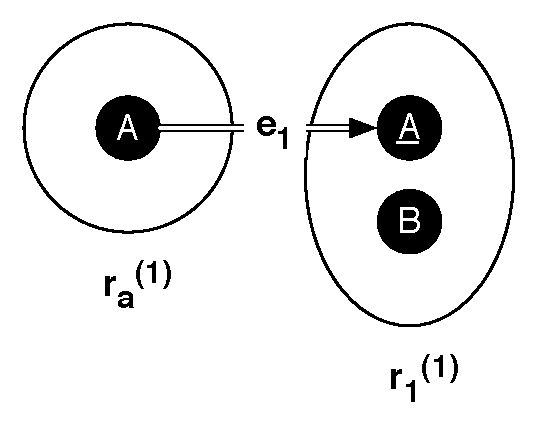
\includegraphics[width=3.2cm]{optimized0.pdf}
  \caption{optimized d-graph for Example~\ref{ex:optimization}}
  \label{fig:optimized}
\end{figure}

\begin{example}\label{ex:optimization-cont}
  Consider the schema and the query from example \ref{ex:optimization},
  % $\R=\{r_1^{io}(A,B),$ $r_2^{oi}(A,B)\}$ and $q(X) ~\la~ r_1(a,X)$
  whose d-graph is shown in Figure~\ref{fig:optimization}.
  Arc~$e_1$ is the only (non-cyclic) candidate strong arc and is, thus, in
  the initial set of strong arcs; arcs $e_2$ and $e_{3}$ are therefore in the
  initial set of deleted arcs.  This is already the greatest fixpoint we were
  looking for, since equations~(\ref{eqn:fixpointStrongMonotone})
  and~(\ref{eqn:fixpointDeletedMonotone}) are satisfied. In particular, arc
  $e_{3}$ remains deleted, since it is dominated by $e_{1}$, which is strong,
  and then $e_2$ is deleted as well, since no black node is reachable by a
  d-path starting with $e_{2}$.
  The intuition is that relation $r_2$ does not have to provide arbitrary values to $r_1$; indeed, due to the join condition
  in $q$, accessing $r_1$ with values provided by $r_2$ would not provide
  tuples that could be used to answer the query $q$.  The optimized d-graph,
  without deleted arcs, and without source $r_2$, is shown in
  Figure~\ref{fig:optimized}; the strong arc $e_1$ is denoted by a double-lined arrow.
\end{example}
























% % We say that a relation is \emph{free} if all of its attributes are free; a
% % source is \emph{free} if all of its nodes correspond to free attributes.
% \begin{definition}\label{def:free-reachable}
% An input node $v$ in a d-graph $G$ is inductively defined as \emph{free-reachable},
% denoted as $\isFreeReachable(v)$, if either
% \begin{enumerate}
% \item there is a weak arc $u\arc v$ in $G$
% such that all input nodes in $u$'s source are free-reachable, or
% 
% \item all strong arcs $u_1\arc v$, $\dots$, $u_n\arc v$ in $G$ are such that all input nodes in $u_i$'s source are free-reachable, for $1\leq i\leq n$.
% \end{enumerate}
% \end{definition}
% Clearly, whenever the query is constant-free (like after the pre-processing step), a relation is queryable only if all of its input nodes are free-reachable.
% %%%
% 
% Let $\isBlack$ be a function that takes a node and returns $\true$ if and only
% if the node is black, and let $\joined$ be a function that takes two nodes and
% returns $\true$ if and only if the corresponding variables are joined in the
% query.
% %
% Based on the above observations, we characterize strong arcs and deleted arcs
% by the following equations~(\ref{eqn:fixpointStrongNonMonotone})
% and~(\ref{eqn:fixpointDeletedNonMonotone}).
% 
% \begin{equation}\label{eqn:fixpointStrongNonMonotone}
%   \begin{array}{rl}
%     \isStrong(u\arc v) = & \lnot \isDeleted(u\arc v) \land{} \\
%     & \isBlack(u) \land \isBlack(v) \land \joined(u,v) \land{} \\
%     & \forall \gamma \in \outArcs(v)
%        (\isStrong(\gamma) \lor \isDeleted(\gamma))
%        %%% DM adds
%        \land{} \\
%        & \isFreeReachable(v)
%        %%%
%   \end{array}
% \end{equation}
% 
% \begin{equation}\label{eqn:fixpointDeletedNonMonotone}
%   \begin{array}{rl}
%     \isDeleted(u\arc v) = & \lnot \isStrong(u\arc v) \land{}\\
%     & [\isBlack(v) \land \exists(u'\neq u) (\isStrong(u'\arc v)) \lor{}\\
%     & \lnot \isBlack(v) \land \forall\gamma \in \outArcs(v) (\isDeleted(\gamma))]
%   \end{array}
% \end{equation}
% 
% 
% %TRA PARENTESI, QUESTA LA POSSO ANCHE SCRIVERE COME
% %\[  \begin{array}{rl}
% %\isDeleted(u\arc v) \equiv & \lnot \isStrong(u\arc v) \land\\
% %& [\isBlack(v) \ra \exists(u'\neq u) (\isStrong(u'\arc v)) \land \\
% %& \lnot \isBlack(v) \ra \forall\gamma \in \outArcs(v) (\isDeleted(\gamma))]
% %  \end{array}
% %\]
% 
% Ideally, for a given d-graph, we aim to determine two maximal sets
% respectively of deleted arcs and strong arcs that satisfy the above equations.
% % reach a solution for these equations that maximizes the number of deleted
% % arcs as well as the number of strong arcs. That these two goals are
% % non-contradictory can be seen as follows.
% Let us call \emph{candidate strong} arc any arc whose nodes are black and whose
% corresponding variables are joined in the query; let us indicate with
% $\arcs(\GqR)$ the set of all arcs in $\GqR$ and with $\candStr(\GqR)$ the set
% of all candidate strong arcs in $\GqR$.
% %%
% Clearly, \myi~only candidate strong arcs have the potential to become strong
% arcs and \myii~no candidate strong arc can ever be deleted, since, by
% definition, it reaches a black node and is never dominated by another strong
% arc (for any given node in $\GqR$, its incoming arcs, if any, are either all
% strong or all weak). Therefore the set of strong arcs and the set of deleted
% arcs must be disjoint; this is reflected in the first conjunct of
% equation~(\ref{eqn:fixpointStrongNonMonotone}) and
% equation~(\ref{eqn:fixpointDeletedNonMonotone}).
% %
% %%% DM adds
% Note also that only those candidate strong arcs that do not destroy
% free-reachability can actually become strong.  In particular, we say that a
% candidate strong arc $u\arc v$ is \emph{circular} if it is contained in a
% d-path $u\dpath u$ such that all arcs in it are candidate strong; we indicate by
% $\circularCand(\GqR)$ the set of circular candidate strong arcs in $\GqR$.
% %%%
% 
% We call the pair $(\S,\D)$ a \emph{solution} for
% equations~(\ref{eqn:fixpointStrongNonMonotone})
% and~(\ref{eqn:fixpointDeletedNonMonotone}) if $\S$ and $\D$ are respectively
% sets of strong arcs and deleted arcs (among the arcs of a given dependency
% graph) that satisfy the conditions of the equations; the solution is
% \emph{maximal} if no other solution $(\S',\D')$ exists such that $\S'\supset
% \S$ or $\D'\supset \D$.
% %%% DM adds
% A solution $(\S,\D)$ can be used to produce a new d-graph ${\GqR}^{(\S,\D)}$,
% that we call \emph{optimized d-graph}, by removing from $\GqR$ all
% arcs in $\D$ and by labeling as ``strong'' all arcs in $\S$, by labeling as
% ``weak'' all remaining arcs (note that the input d-graph $\GqR$ had no
% explicit arc labeling), and, finally, by removing all nodes with no incoming or
% outgoing arcs and all sources with no nodes.
% %%%
% It turns out that there always exists a unique maximal solution for
% equations~(\ref{eqn:fixpointStrongNonMonotone})
% and~(\ref{eqn:fixpointDeletedNonMonotone}).
% 
% \begin{lemma}\label{lem:free-reachability}
%   Let $(\S,\D)$ be a solution for~(\ref{eqn:fixpointStrongNonMonotone}')
%   and~(\ref{eqn:fixpointDeletedNonMonotone}) for a d-graph $G$, where
%   (\ref{eqn:fixpointStrongNonMonotone}') is as
%   (\ref{eqn:fixpointStrongNonMonotone}), but without the last conjunct. An input
%   node $u$
%   % of a queryable source
%   is free-reachable in $\GSD$ iff there is no d-path $u\dpath u$ in $\GSD$
%   consisting only of strong arcs.
% \end{lemma}
% \begin{proof}$ $
% 
% \textit{If part}.
% %If a bound node $u$ (of a queryable source) is not free-reachable then there exist a circular d-path consisting of strong arcs that touches $u$.
% %I then assume that there are no such cycles and I prove that all bound nodes are free-reachable.
% Each input node in $\GSD$ has at least an incoming arc originating in an output node.
% Therefore, if there are no cycles, for queryability, each d-path must eventually originate in a source entirely free.
% If there are cycles, these cannot consist, by hypothesis, of only strong arcs. Then they must contain at least a weak arc, therefore
% 1) necessarily, all arcs in the cycle are weak (else we would have a strong arc followed by a weak arc in a d-path, which is not possible), and 
% %2) each source in the cycle has at least a bound node and a free node (trivially, else it would not be possible to have a cycle, i.e., the source could not have both incoming and outgoing arcs).
% 2) all input nodes of each source in the cycle are free-reachable. Since each input node $u$ necessarily has incoming weak arcs, then it must have all possible incoming weak arcs, from all output nodes with the same attribute. But at least one of these belongs to a source that is free or whose input nodes are all free-reachable, otherwise $u$'s source would not be queryable, against the hypotheses.
% 
% \textit{Only-if part}.
% We prove the contrapositive of this part, i.e., if there is a d-path $u\dpath u$ in $\GSD$ consisting only of strong arcs then $u$ is not free-reachable.
% % We observe that, in order to have a circular d-path, each source in the cycle has at least a bound node and a free node, else it would not be possible to have a cycle, i.e., the source could not have both incoming and outgoing arcs.
% Indeed, according to definition \ref{def:free-reachable}, $u$ is, inductively, free-reachable only if $u$ is free-reachable; however, there is no base case activating the inductive chain, so $u$ is not free-reachable.
% \end{proof}
% \begin{theorem}\label{the:GFP-exists-unique}
%   Equations~(\ref{eqn:fixpointStrongNonMonotone})
%   and~(\ref{eqn:fixpointDeletedNonMonotone}) admit a unique maximal
%   solution for any d-graph $G$.
% \end{theorem}
% %
% \begin{proof}
% We first prove that a solution exists.  Consider
% equations~(\ref{eqn:fixpointStrongMonotone})
% and~(\ref{eqn:fixpointDeletedMonotone}).
% 
% \begin{equation}\label{eqn:fixpointStrongMonotone}
%   \begin{array}{rl}
%     \isStrong(u\arc v) \equiv %& \isStrong(u\arc v) \land \\
%     & \isBlack(u) \land \isBlack(v) \land \joined(u,v) \land \\
%     & \forall \gamma \in \outArcs(v) (\isStrong(\gamma) \lor \isDeleted(\gamma))
%   \end{array}
% \end{equation}
% 
% \begin{equation}\label{eqn:fixpointDeletedMonotone}
%   \begin{array}{rl}
%     \isDeleted(u\arc v) \equiv %& \isDeleted(u\arc v) \land\\
%     & [\isBlack(v) \land \exists u' (\isStrong(u'\arc v)) \lor \\
%     & \lnot \isBlack(v) \land \forall\gamma \in \outArcs(v) (\isDeleted(\gamma))]
%   \end{array}
% \end{equation}
% 
% They induce the definition of two corresponding monotonic fixpoint operators
% $T_{S}$ and $T_{D}$.  This in turn guarantees the existence of the greatest
% fixpoint for~(\ref{eqn:fixpointStrongMonotone})
% and~(\ref{eqn:fixpointDeletedMonotone}) (the one that maximizes the number of
% strong arcs and deleted arcs), for any given initial sets of strong arcs and of
% deleted arcs.
% 
% %%% DM adds
% % We observe that a bound node $u$ of a queryable source is free-reachable in
% % $\GqR$ if and only if there does not exist a d-path $u\dpath u$ in $\GqR$
% % consisting only of strong arcs.
% By Lemma \ref{lem:free-reachability},
% %%%
% the largest set of strong arcs one can hope for is
% $\S^{0}=\candStr(G)\setminus\circularCand(G)$, whereas the largest achievable
% set of deleted arcs is its complement $\D^{0}=\arcs(G)\setminus\S^{0}$;
% clearly, $\S^{0}$ and $\D^{0}$ are disjoint.
% %%
% It now suffices to observe that the fixpoint $(\S^{\omega},\D^{\omega})$ for
% equations~(\ref{eqn:fixpointStrongMonotone})
% and~(\ref{eqn:fixpointDeletedMonotone}) obtained via $T_{S}\circ T_{D}$
% starting from $(\S^{0},\D^{0})$ is necessarily also a solution for
% equations~(\ref{eqn:fixpointStrongNonMonotone})
% and~(\ref{eqn:fixpointDeletedNonMonotone}), since, by monotonicity, $\S^{0}\cap
% \D^{0}=\emptyset$ entails that $\S^{\omega}\cap \D^{\omega}=\emptyset$, so all
% conditions in~(\ref{eqn:fixpointStrongNonMonotone})
% and~(\ref{eqn:fixpointDeletedNonMonotone}) are satisfied,
% %%% DM adds
% including free-reachability by Lemma \ref{lem:free-reachability}.
% 
% To see that the maximal solution for~(\ref{eqn:fixpointStrongNonMonotone})
% and~(\ref{eqn:fixpointDeletedNonMonotone}) is unique and coincides with
% $(\S^{\omega},\D^{\omega})$, let us assume, by contradiction, that there is
% another solution $(\S',\D')$ such that $\S'\supset \S^{\omega}$ or $\D'\supset
% \D^{\omega}$. However, since $(\S',\D')$ is a solution, we have $\S'\cap
% \D'=\emptyset$. Besides, $\S'\subseteq \S^{0}$, since only
% %%% DM adds
% non-circular
% %%%
% candidate strong arcs can be strong arcs, and $\D'\subseteq \D^{0}$, since no
% candidate strong arc can be deleted, as was argued before. This means that
% $(\S',\D')$ would also be a solution for
% equations~(\ref{eqn:fixpointStrongMonotone})
% and~(\ref{eqn:fixpointDeletedMonotone}), contradicting the fact
% that~(\ref{eqn:fixpointStrongMonotone}) and~(\ref{eqn:fixpointDeletedMonotone})
% are guaranteed to have a unique greatest fixpoint.
% %%
% \end{proof}
% 
% Theorem \ref{the:GFP-exists-unique} indicates that we can always find the
% largest sets of strong arcs and of deleted arcs possible for a given dependency
% graph.
% %
% We present in Figure~\ref{fig:algoBP} an algorithm that determines such sets
% according to the above criteria.  The algorithm calculates the initial sets of
% strong arcs (the
% %%% DM adds
% non-circular
% %%%
% candidate strong arcs) and deleted arcs (its complement) and
% then implements the $T_{S}$ and $T_{D}$ monotonic fixpoint operators used in
% the proof of Theorem \ref{the:GFP-exists-unique} and applies them to the sets
% until a fixpoint is reached. This is stated below in Theorem
% \ref{the:algoCorrectness}, which trivially holds.
% 
% \begin{theorem}\label{the:algoCorrectness}
%   The function \textit{calculateGFP}($G$) shown in Figure~\ref{fig:algoBP}
%   computes the maximal solution for
%   equations~(\ref{eqn:fixpointStrongNonMonotone})
%   and~(\ref{eqn:fixpointDeletedNonMonotone}) \wrt d-graph $G$.
% \end{theorem}
% %
% Termination of the algorithm is guaranteed by the monotonicity of the fixpoint
% operators induced by equations~(\ref{eqn:fixpointStrongMonotone})
% and~(\ref{eqn:fixpointDeletedMonotone}), which are implemented by the functions
% \textit{unmarkStrong} and \textit{unmarkDeleted} respectively. The monotonicity
% also ensures that the algorithm runs in polynomial time in the size of the
% d-graph.
% %
% \begin{theorem}\label{the:algoComplexity}
%   \textit{calculateGFP}$(G)$ runs in polynomial time in the size of $G$.
% \end{theorem}
% 
% \begin{figure}[t]
% \centering
% \begin{tabular}{l}
% \textit{calculateGFP}($G$ : d-graph) : arc set $\times$ arc set\\
% \quad$\S$ := $\candStr(G)\setminus\circularCand(G)$\\
% \quad$\D$ := $\arcs(G)\setminus\S$\\
% \quad\codedo \{\\
% 	\quad\quad($\S'$,$\D'$) := ($\S$,$\D$)\\
% 	\quad\quad$\S$ := unmarkStrong($\S'$,$\D'$,$G$)\\
% 	\quad\quad$\D$ := unmarkDeleted($\S'$,$\D'$,$G$)\\
% \quad\} \codewhile ($\S$,$\D$) $\neq$ ($\S'$,$\D'$)\\
% \quad\codereturn ($\S'$,$\D'$)\\
% \\
% \textit{unmarkStrong}($\S$ : arc set, $\D$ : arc set, $G$ : d-graph) : arc set\\
% 	\quad$\S'$ := $\S$\\
% 	\quad\codeforeach arc $u\arc v\in \S$\\
% 		\quad\quad\codeforeach arc $\gamma\in \outArcs(v,G)$\\
% 			\quad\quad\quad\codeif ($\gamma\not\in\S\cup\D$) $\S'$ := $\S'\setminus\{u\arc v\}$; \codebreak\\
% %			\textbf{end if}\\
% %		\textbf{end for}\\
% %	\textbf{end for}\\
% 	\quad\codereturn $\S'$\\
% \\
% \textit{unmarkDeleted}($\S$ : arc set, $\D$ : arc set, $G$ : d-graph) : arc set\\
% 	\quad$\D'$ := $\D$\\
% 	\quad\codeforeach arc $u\arc v\in\D$\\
% 		\quad\quad\codeif ($\isBlack(v)$) \codethen\\
% 			\quad\quad\quad\codebool strongExists := \codefalse\\
% 			\quad\quad\quad\codeforeach arc $u' \arc v'\in\S$\\
% 				\quad\quad\quad\quad\codeif ($v = v'$) \codethen strongExists := \codetrue; \codebreak\\
% %				\textbf{end if}\\
% %			\textbf{end for}\\
% 			\quad\quad\quad\codeif (\textbf{not} strongExists) \codethen $\D'$ := $\D'\setminus\{u\arc v\}$\\
% %			\textbf{end if}\\
% 		\quad\quad\codeelse \textit{($v$ is white)}\\
% 			\quad\quad\quad\codeif $(\outArcs(v,G)\setminus\D\neq\emptyset)$ \codethen $\D'$ := $\D'\setminus\{u\arc v\}$\\
% %				\textbf{end if}
% %			\textbf{end for}
% %		\textbf{end if}
% %	\textbf{end for}
% 	\quad\codereturn $\D'$
% \end{tabular}
%   \caption{Algorithm determining the maximal sets of strong arcs and deleted arcs}
%   \label{fig:algoBP}
% \end{figure}
% 
% % The sets of arcs $(\S,\D)$ returned by the function
% % \textit{calculateGFP}($\GqR$) can be used to produce a new d-graph, that we
% % call \emph{optimized d-graph}, by removing from $\GqR$ all arcs in $\D$ and
% % by labeling as ``strong'' all arcs in $\S$, by labeling as ``weak'' all
% % remaining arcs (note that the input d-graph $\GqR$ had no explicit arc
% % labeling), and, finally, by removing all nodes with no incoming or outgoing
% % arcs and all sources with no nodes. Then
% 
% \begin{example}\label{ex:optimization}
%   Let $\R=\{r_1(\battr{A},B), r_2(A,\battr{B})\}$ be a set of relational
%   schemata and $q(X) ~\la~ r_1(a,X)$ a query over $\R$.  The d-graph $\GqR$ for
%   $q$ is shown in Figure~\ref{fig:optimization}, where we have named the
%   sources as the corresponding relations, with a superscript indicating the
%   occurrence number of that relation in the query.  We first eliminate the
%   constant $a$ occurring in $q$ by introducing a new relation $r_a$ with domain
%   $A$ and populated by the single tuple $\tup{a}$ and by rewriting $q$ as
%   follows:
%   \[
%     q(X) ~\la~ r_{a}(Y), r_1(Y,X).
%   \]
%   Arc~$e_1$ is the only (non-circular) candidate strong arc and is, thus, in
%   the initial set of strong arcs; arcs $e_2$ and $e_{3}$ are therefore in the
%   initial set of deleted arcs.  This is already the greatest fixpoint we were
%   looking for, since equations~(\ref{eqn:fixpointStrongMonotone})
%   and~(\ref{eqn:fixpointDeletedMonotone}) are satisfied. In particular, arc
%   $e_{3}$ remains deleted, since it is dominated by $e_{1}$, which is strong,
%   and then $e_2$ is deleted as well, since no black node is reachable by a
%   d-path starting with $e_{2}$.  The intuition is that relation $r_1$ does not
%   have to provide arbitrary values to $r_2$; indeed, due to the join condition
%   in $q$, accessing $r_1$ with values provided by $r_2$ would not provide
%   tuples that could be used to answer the query $q$.  The optimized d-graph,
%   without deleted arcs, and without source $r_2$, is shown in
%   Figure~\ref{fig:optimized}; the strong arc $e_1$ is denoted by a solid line.
%   %%
% \end{example}
% 
% \begin{figure}[t]
%   \centering
%   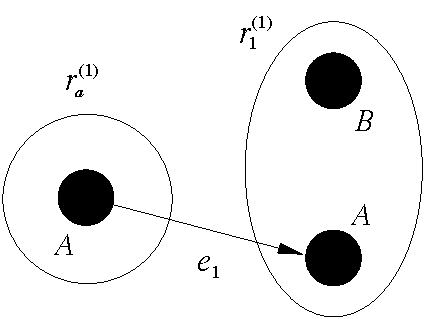
\includegraphics[width=3.2cm]{optimized.pdf}
%   \caption{optimized d-graph for Example~\ref{ex:optimization}}
%   \label{fig:optimized}
% \end{figure}
% 
% 
% \subsection{Properties of dependency graphs}
% 
% Now we prove a series of results that illustrate the correspondence between the
% dependency graph and the extraction process; with these results we
% prove soundness and completeness of the optimization algorithm.
% 
% \begin{lemma} \label{lem:extraction-tree}
%   Consider a relational schema $\R$, a database $\D$ for $\R$ and a query $q$ over
%   $\R$. A tuple $t_0$ can be extracted in $k$ steps from relation $r_{0}\in\R$ if and only
%   if we can construct a tree, called \emph{extraction tree}, whose nodes are
%   tuples in $\D$, such that:
%   \begin{enumerate}
%   \item $t_0$ is the root;
%   \item the leaves of the tree are tuples belonging to free relations of $\R$;
%   \item if $t$ is a tuple belonging to a non-free relation $r\in\R$, let $\dd{X}{m}$
%     be the input attributes of $r$; then $t$ has $n$ children $\dd{t}{n}$, with
%     $n \leq m$, such that $t_i$ belongs to relation $r_i$, and the values
%     $t[X_1],\ldots,t[X_m]$ belong to the set of all values in $\dd{t}{n}$
%     corresponding to output attributes of $\dd{r}{n}$;
%   \item the tree has depth $k$.
%   \end{enumerate}
% \end{lemma}
% 
% \begin{proof}
%   
%   \onlyifdirection The proof is by induction on the number of iterations needed
%   for extracting $t_0$, starting from the free relations.
%   
%   \textit{Base step.} At the base step, $t_0$ belongs to a free source, and the
%   extraction tree is constituted by $t_0$ only.
%   
%   \textit{Inductive step.} Let $\dd{t}{p}$ be all tuples that can be extracted in at most
%   $k-1$ steps.
%   By the induction hypothesis, we have that $\dd{t}{p}$ are
%   roots of extraction trees with depth less than or equal to $k-1$.
%   Since $t_0$ is extracted in one more step, the values $t_0[X_1],\ldots,t_0[X_m]$,
%   corresponding to the input attributes of $r_0$, are found in tuples
%   $\dd{t}{p}$, in correspondence of the output attributes of the
%   relations $\dd{{r}}{p}$ to which $\dd{{t}}{p}$ belong respectively;
%   at least one of these values is found in a tuple that requires $k-1$ extraction steps (and thus has a corresponding extraction tree of depth $k-1$), otherwise $t_{0}$ could be extracted in less than $k$ steps.
%   Consider the tree having $t_0$ as root and $\dd{{t}}{p}$ (with the respective extraction trees) as children of $t_0$.
%   Such a tree has depth $k$ and it is immediate to verify that it satisfies the properties of an extraction tree.
%   
%   \ifdirection Consider an extraction tree of depth $k$ having $t_0$ as root.
%   It is easy to see that, starting from the leaves of the tree, immediately
%   accessible because they belong to free relations by construction, the root
%   $t_0$ is extracted in $k$ iterations.  Indeed, because of the properties of
%   the tree, at each step, the values of tuples of level $i$ are sufficient to
%   access the tuples at level $i-1$, until the root is eventually extracted.
%   Observe that, since the tree is arbitrary in this case, the root could in
%   principle be extracted in a number of iterations less than $k$.
% \end{proof}
% 
% Now we come to the correspondence between the dependency graph and the
% extraction trees.  
% 
% %Now we consider the query plans, expressed in Datalog notation, constructed as
% %specified before, on the basis of the dependency graph.
% 
% \begin{lemma} \label{lem:graph-vs-extraction}
%   Given a relational schema $\R$, a database $\D$ for $\R$ and a query $q$
%   over $\R$, let $\GqR$ be the dependency graph for $q$.  Let $t_0$ be a tuple
%   obtainable from relation $r_0$;
%   %with a query plan as above;
%   then if $t_1$ is a child of $t_0$ in the extraction tree for $t_0$, with
%   $t_1$ belonging to relation $r_1$, we have that if the value $t_1[A_1]$ is used
%   to extract $t_0$, with $t_1[A_1]=t_0[A_0]$ (where $A_0$ and $A_1$ are
%   attributes of $r_0$ and $r_1$ respectively), then there is an arc from $A_1$
%   to $A_0$ in $\GqR$.  In this case, we say that the extraction tree
%   \emph{covers} the arc $(A_1,A_0)$,
% \end{lemma}
% 
% \begin{proof}
%   Trivial, since $A_1$ and $A_0$ must belong to the same abstract domain, $A_1$
%   is an output attribute and $A_0$ is an input attribute.
% %  , and the Datalog program encoding the extraction
% %  process is constructed according to the arcs in $\GqR$.
% \end{proof}
% 
% The above lemma, which is quite straightforward, states that the d-graph constitutes a structure on which all extraction trees are obliged to lie.
%  By pruning the d-graph we therefore forbid the possibility of
% having certain extraction trees (and therefore certain extraction processes).
% We shall prove that the pruning of the d-graph does not exclude any
% answer to the query, for all possible source databases.
% %
% %  We will start by
% %showing that an optimized extraction tree enjoys certain properties, that are
% %presented in the following proposition.
% %
% An optimized d-graph generated via the result of the function
% \textit{calculateGFP} trivially has the properties stated in
% Proposition~\ref{pro:dependency-graph} below.
% 
% \begin{proposition}\label{pro:dependency-graph}
%   Consider an optimized d-graph $\GqR$ for a query $q$ over a set $\R$ of
%   relational schemata.  We have that $\GqR$ has the following properties.
%   \begin{enumerate}
%   \item From each node in $\GqR$ it is possible to reach a black node through a
%     d-path.
%   \item For each node $u$, its incoming arcs, if any, are either all strong or
%     all weak.
%   \item There is no d-path that traverses a strong arc and
%     successively a weak arc.
%   \item From every node of $\GqR$, a free source is reachable through a d-path
%     in reverse direction.
%   \end{enumerate}
% \end{proposition}
% 
% With the previous results in place, we are finally able to prove the soundness
% and completeness of our optimization, i.e. that the pruning of the arcs of the
% d-graph removes as many arcs as possible, while still retaining the
% possibility of retrieving all obtainable tuples from the relations (and therefore
% obtaining all obtainable answers from the optimized query plan) with a query
% plan based on the optimized d-graph.
% 
% \begin{theorem} \label{the:optim-soundness}
%   Consider a relational schema $\R$, a database $\D$ for $\R$, a query $q$
%   over $\R$, the d-graph $\GqR$ for $q$ and an arc $u\arc v$ in
%   $\GqR$, removed by the optimization procedure \textit{calculateGFP}$(\GqR)$.
%   For each tuple $\theta$ in the answer to $q$, we have that $\theta$ is the root of an extraction tree that does not cover $u\arc v$.
% \end{theorem}
% 
% \begin{proof}
%   The removal of $u\arc v$ can happen for two reasons:
%   \begin{enumerate}
%   \item $v$ is a black node with an incoming strong arc $u'\arc v$ different from $u\arc v$.
%   \item $v$ is a white node and all arcs in $\outArcs(v)$ are also deleted.
%   %$u\arc v$ is outgoing or incoming from a node that is deleted
%    % because no black node is reachable from it to a dependency path;
%   \end{enumerate}
%   
%   Consider any tuple $t$ belonging to a relation $r$
%   appearing in $q$, used to construct the answer $\theta$, and an extraction
%   tree with $t$ as root.  If such a tree does not cover $u\arc v$, we are
%   done.  
%   
%   \textit{Case 1.} Instead, assume that $u\arc v$ is covered by the tree. We know that
%   there is an arc $u'\arc v$ that is strong.  Let $A, B, A'$ be the
%   attributes labelling $u, v, u'$ respectively; let $r_{u}, r_v, r_{u'}$ be
%   the relations of $A, B, A'$ respectively, and $t_{u}, t_v, t_{u'}$ the
%   corresponding tuples in the tree.  From the covering we have
%   $t_{u}[A]=t_v[B]$, and by the properties of strong arcs we have
%   $t_{u'}[A]=t_v[B]$ (note that because of the join condition between $r_{u'}$
%   and $r_v$ the tuple $t_{u'}$ must belong to the extraction tree of which $t$ is
%   the root).  Therefore, if we prune the subtree having $t_{u}$ as root, we still
%   have an extraction tree for $t$.
% 
%   \textit{Case 2.} Assume first that $outArcs(v,\GqR)=\emptyset$. Here, no black node, including those corresponding to $r$'s attributes, is reachable from $v$ through a d-path in $\GqR$. Therefore, by the contrapositive of Lemma \ref{lem:graph-vs-extraction}, no extraction tree with root $t$ can cover an arc outgoing from $v$. Consequently, such a tree cannot cover $u\arc v$ either, since $v$ cannot be a node for the root ($v$ is white) and no arcs outgoing from $v$ can be covered.
%   Assume now that $outArcs(v,\GqR)=\Gamma\neq\emptyset$. Each arc $\gamma\in\Gamma$ is deleted by the algorithm. If there is no circular d-path in $\GqR$ containing $\gamma$, $\gamma$ will, inductively, by following all outgoing arcs, end up either in case 1 or in case 2 with no outgoing arcs. Therefore the thesis holds for all arcs in $\Gamma$, i.e., there is an extraction tree with root $t$ not covering any of the arcs outgoing from $v$. But then, such a tree cannot cover $u\arc v$ either, for the same reasons as in the previous case. If there is one (or more) circular d-path of the form $u_{1}\arc v_{1},\dots,u_{n}\arc v_{n}=u_{1}$ in $\GqR$ containing $\gamma$, each arc $u_{i}\arc v_{i}$ is deleted by the algorithm and, if we exclude the circular d-paths that contain it, will also, inductively, end up either in case 1 or in case 2 with no outgoing arcs. The circular d-paths can then be disregarded, since they do not provide any way of constructing tuples for nodes outside $\{u_{1},\dots,u_{n}\}$.
% \end{proof}
% 
% 
% 
% \begin{theorem} \label{the:optim-completeness}
%   Consider a relational schema $\R$, a query $q$ over $\R$, the dependency graph
%   $\GqR$ for $q$ and an arc $u\arc v$ in $\GqR$, that is \emph{not} removed
%   by the optimization procedure.  Then there exists a database $\D$ for
%   $\R$ such that a tuple $\theta$ in the answer to $q$ is constructed with tuples $\dd{t}{h}$
%   (extracted from sources that have black attributes in $\GqR$) such that one of the $t_i$ (with $1 \leq i \leq h$) has an extraction tree
%   covering $u\arc v$ on tuples $t_{u}$ and $t_{v}$, respectively,
%   and no sound query planner can build extraction trees to construct $\theta$ without extracting $t_{u}$ and $t_{v}$.
% %  
% %  such that removing $u_1\arc u_2$ the tree does not
% %  satisfy the properties of an extraction tree any more.
% \end{theorem}
% 
% \begin{proof}
%   We exhibit database $\D$ such that $q$ has
%   a single answer, $\theta$, that is not returned if $t_{u}$ and $t_{v}$ are not extracted.
%   We start by ``freezing'' the atoms of $q$: we assign to each variable $X$ a
%   distinct value $\psi(X)$, and for each atom $r(\dd{X}{m})$ in $q$ we add the fact
%   $r(\psi(X_1),\ldots,\psi(X_m))$ to $\D$.  In this way, the distinguished
%   variables of $q$ can be mapped to $\theta$.  Then we
%   iteratively construct an extraction tree for each of the $h$ tuples inserted, such that the following four properties are verified.  Consider an inserted fact
%   $r(\dd{c}{m})$ and its corresponding tuple $t$, and let $\ddd{A}{i}{p}$ be its input
%   attributes; add children to the tree such that:
%   \begin{enumerate}
%   \item if $A_{i_j}$, with $1 \leq j \leq p$, has weak incoming arcs, then
%     $c_{i_j}=t[A_{i_j}]$ appears exactly once in the children of $t$;
%   \item if $A_{i_j}$, with $1 \leq j \leq p$, has $k$ strong incoming arcs
%     $B_1\arc A_{i_j},\ldots,B_k\arc A_{i_j}$ in $\GqR$, then $c_{i_j}$ appears $k$
%     times in the children of $t$, in correspondence of $\dd{B}{k}$;
%   \item all other values in the children of $t$ are newly introduced values;
%   \item the arc $u\arc v$ is eventually covered.
%   \end{enumerate}
%   Note that this is always possible since, by
%   Proposition~\ref{pro:dependency-graph} (property~2), each node in $\GqR$ has
%   incoming arcs that are either all weak or all strong, and moreover
%   $u\arc v$ can be covered because of property~1 of
%   Proposition~\ref{pro:dependency-graph}.  The trees can be completed because
%   of Lemma~\ref{lem:extraction-tree}.
%   At this point, we have a database $\D$
%   constituted only by the facts of the extraction trees having as roots the
%   facts obtained by ``freezing'' the atoms of $q$.
%   %; $\theta$ is an answer to $q$ in $D$, constructed with tuples $\dd{t}{h}$ extracted by $\dd{\T}{h}$, respectively.
%   %
%   Let $\T_{i}$, $1\leq i\leq h$, be the extraction tree with root $t_{i}$ covering $u\arc v$ on $t_{u}$ and $t_{v}$, and let $c_{u}$ and $c_{v}$ be the corresponding values carried by $u$'s and $v$'s attribute, respectively.
%   %Then, no extraction tree not covering $u\arc v$ that can be built by a sound query planner exists that extracts $t_{i}$ from $D$.
%   If $v$ has weak incoming arcs or exactly one strong incoming arc, the input attributes of $v$'s relation cannot receive binding values, so no extraction tree not covering $u\arc v$ exists that extracts $t_{i}$ from $D$.
%   If $v$ has at least one strong incoming arc $u'\arc v$ besides $u\arc v$, then $t_{i}$ can be extracted by an extraction tree not covering $u\arc v$, since by construction there is a tuple in which $u'$'s attribute will also carry value $c_{u}$; however, it cannot be known whether $\theta$ is an answer to $q$ unless a tuple $\overline{t}_{u}$ for $u$'s relation is in $D$ such that $\overline{t}_{u}[A_{u}]=t_{u}[A_{u}]$, where $A_{u}$ is $u$'s attribute, i.e., $t_{u}$ needs to be extracted.
% \end{proof}
% 
% As a straightforward consequence of Theorems \ref{the:optim-soundness} and \ref{the:optim-completeness}, the optimized d-graph only makes use of relevant relations.
% %
% \begin{theorem}\label{the:dgraph-relevant}
%   Let $\GqR$ be an optimized d-graph for a CQ $q$ over a relational schema $\R$.
%   A relation $r\in\R$ is relevant iff
%   \myi $r$ is nullary and occurs in $q$, or
%   \myii $r$ occurs in $\GqR$.
% \end{theorem}
% %
% In other words, theorem \ref{the:dgraph-relevant} states that the d-graph gives us a procedure for deciding relevance of a relation in the context of CQs.

% \subsection{Generation of a query plan}
% 
% Now we come to the construction of the query plan.  From the resulting
% optimized d-graph we construct the optimized query plan, expressed in
% Datalog notation, as shown in the algorithm of Figure \ref{fig:algoQueryPlan}.
% %
% %%% DM adds
% The Datalog program is evaluated according to the usual least fixpoint
% semantics; it is guaranteed by construction that the least fixpoint can be
% calculated by only making valid accesses.
% %%%
% 
% \begin{figure}[t]
% INPUT: optimized d-graph $\GqR$, query $q$, relations $\R$\\
% OUTPUT: a Datalog program corresponding to the optimized query plan\\
% \begin{enumerate}
% \item [1]Rewrite $q$ as follows:
%   \begin{enumerate}
%   \item [1.1]The query head is the same
%   \item [1.2]Each atom in $q$'s body is replaced by an atom with the same
%     arguments but with a fresh new relation name, henceforth used to uniquely
%     identify the corresponding source
%   \end{enumerate}
% \item [2]For each atom $p$ of arity $n$
% %(X_{1},\dots,X_{n})$
%  in the body of the rewritten
%   query $q$
%   %%% DM adds
%   or in the schema of a relation not in $q$ with incoming or outgoing arcs,
%   %%%
%   a rule is generated as follows:
%   \begin{enumerate}
%   \item [2.1]The head atom is $p(Y_{1},\dots,Y_{n})$, where the $Y_{i}$'s are
%     fresh new variables
%   \item [2.2]The body has one atom $r(Y_{1},\dots,Y_{n})$, where $r$ is the
%     name of the relation corresponding to $p$'s source
%   \item [2.3]The body also has one atom for each bound node $v$ in $q$'s head
%     with incoming arcs:
%     \begin{enumerate}
%     \item [2.3.1]The atom has a fresh new relation name that uniquely
%       identifies $v$ and only 1 argument containing the variable corresponding
%       to $v$ in the head
%     \item [2.3.2]If $v$'s incoming arcs are weak, create one new rule for each
%       arc $u\arc v$ as follows:
%       \begin{enumerate}
%       \item [2.3.2.1]The head is the atom created in step 2.3.1
%       \item [2.3.2.2]The body has one atom. The relation name is $u$'s source
%         identifier.  All positions in the atom have a new variable, except for
%         the position corresponding to $u$, which has the same variable as the
%         one in the head
%       \end{enumerate}
%     \item [2.3.3]If $v$'s incoming arcs are strong, create one new rule.
%       \begin{enumerate}
%       \item [2.3.3.1]The head is the atom created in step 2.3.1
%       \item [2.3.3.2]The body has one atom for each arc $u\arc v$. The relation
%         name is $u$'s source identifier.  All positions in the atom have a new
%         variable, except for the position corresponding to $u$, which has the
%         same variable as the one in the head
%       \end{enumerate}
%     \end{enumerate}
%   \end{enumerate}
% \end{enumerate}
% \caption{Algorithm producing the Datalog program corresponding to the optimized
%  query plan}
%   \label{fig:algoQueryPlan}
% \end{figure}
% 
% The algorithm rewrites the original query over new versions of the relations in
% the body. For each predicate $r$ in the body of the query, we introduce a new
% predicate with the same arity as $r$ that acts as a sort of \emph{cache} in
% which we store, during the query answering process, all the tuples extracted
% from $r$.  This is done in step~1.2 of the algorithm of
% Figure~\ref{fig:algoQueryPlan}. Note that different occurrences of the same
% predicate give rise to different names; in the examples we choose, e.g., to add
% a hat symbol to the predicate name as well as an occurrence number.
% 
% Each cache relation is defined in step~2 of the algorithm as the corresponding
% original relation, but where each bound variable receives its binding values
% from another new relation created for that purpose in step~2.3.  Such relation
% takes into account the arcs in the d-graph: if the corresponding
% incoming arcs are weak (resp., strong), then in step~2.3.2 (resp., step~2.3.3)
% the relation is defined as a disjunction (resp., conjunction) of the cache
% relations corresponding to the origin nodes, since any of them (resp., only
% their join) can provide binding values.
% 
% Finally, the program generated by the algorithm of
% Figure~\ref{fig:algoQueryPlan} is completed by adding a fact for each relation
% created in the preprocessing step~to eliminate the constants from the query;
% the fact has the form $r_{a}(a)$, where $r_{a}$ is the created relation and $a$
% is the removed constant.
% 
% \begin{example}\label{exa-query-plan}
%   We refer to Example~\ref{ex:optimization}. From the optimized dependency
%   graph relative to $q$, the algorithm of Figure~\ref{fig:algoQueryPlan}
%   generates the following plan:
%   \[
%     \begin{array}{rcl}
%       q(X) &\la& \retr{r}_a^{1}(X),\retr{r}_1^{1}(X,Y)\\
%       \retr{r}_a^{1}(X_{1}) &\la& r_a(X_{1})\\
%       % \retr{r}_1^{1}(X_{2},Y_{2}) &\la&
%       % r_1(X_{2},Y_{2}),\retr{r}_a^{1}(X_{2})\\
%       \retr{r}_1^{1}(X_{2},Y_{2}) &\la& r_1(X_{2},Y_{2}),s^{X_{2}}(X_{2})\\
%       s^{X_{2}}(X_{2}) &\la& \retr{r}_a^{1}(X_{2})\\
%       r_{a}(a) &\la&\\
%     \end{array}
%   \]
%   In this example, the support relation $s^{X_{2}}$ introduced by step~2.3.3 is
%   defined as $r_{a}^{1}$, since there is only one corresponding incoming strong
%   arc. The third and fourth rules could therefore more simply be written as the
%   following single rule:
%   \[
%     \begin{array}{rcl}
%       \retr{r}_1^{1}(X_{2},Y_{2}) &\la&
%       r_1(X_{2},Y_{2}),\retr{r}_a^{1}(X_{2})\\
%     \end{array}
%   \]
%   The Datalog program above shows that relation $r_{2}$, which could in
%   principle provide useful values to $r_{1}$, is not needed at all to answer
%   the query because of the join between $r_{a}$ and $r_{1}$.
%   %%
% \end{example}
% 
% Such a Datalog program ensures that the binding values for the bound positions
% of a relation $r$ are obtained from values retrieved from the appropriate
% relations and stored in the caches. Essentially, it defines a procedure to construct extraction
% trees; such trees necessarily cover only the arcs of the pruned dependency
% graph. 
% 
% \medskip
% 
% We now state that the optimized query plan generated by our approach is both
% sound, i.e., it returns only tuples that are in the answer to the query, and
% complete, i.e., it does not miss any obtainable tuple, taking into account the
% binding patterns.
% Moreover, such query plan is extraction-minimal, i.e., there is at least a database in which all tuples extracted by it are necessary.
% %
% \begin{definition}\label{def:extraction-minimality}
% Let $q$ be a query over a relational schema $\R$.
% A tuple $t$ in a database $\D$ for $\R$ is \emph{necessary} to obtain a tuple $\theta$ in the answer to $q$ for $\D$ if no sound query plan exists that obtains $\theta$ without extracting $t$.
% A sound query plan $\Pi$ is \emph{extraction-minimal} if there exists a database $D$ for which all tuples extracted by $\Pi$ are necessary to obtain some answer tuple.
% \end{definition}
% 
% %%% DM removes
% % Besides, the plan minimizes the accesses to the relations.
% %%%
% %
% \begin{theorem}\label{thm-soundness-and-completeness}
%   Let $q$ be a query over a set $\R$ of relational schemata, and let $\GqR$ be
%   its d-graph and $G=\textit{calculateGFP}(\GqR)$ the corresponding optimized
%   d-graph.
%   Then, the Datalog program $\Pi$ constructed from $q$ by the algorithm in
%   Figure~\ref{fig:algoQueryPlan}, based on $G$, computes all the answers to $q$
%   obtainable from the relations in $\R$, given the binding patterns on them;
%   $\Pi$ is extraction-minimal.
% \end{theorem}
% \begin{proof}
% Soundness (i.e., $\Pi$ returns only tuples that are in the answer to $q$), 
% follows from the fact that the query is reformulated on the caches, which in turn are, by construction,
% a subset of the original relations.
% 
% Completeness (i.e., $\Pi$ does not miss any obtainable answer), follows straightforwardly from Theorem \ref{the:optim-soundness}.
% 
% Extraction-minimality follows trivially from Theorem \ref{the:optim-completeness}.
% \end{proof}
% %
% %%% DM removes
% % This can be proved by showing a correspondence between the accesses of the
% % extraction process and the d-paths in the optimized dependency graph.

% \section{Extensions to more expressive query languages}\label{sec:extensions}

\subsection{Unions of conjunctive queries}
In this section, we address the problem of finding a query plan for a UCQ.
Our approach is to transform a UCQ into an appropriate CQ to which the technique presented can be applied.
The obtained CQ can then be used to determine the relevant relations for the original UCQ.
We assume in the following, w.l.o.g., that the initial UCQ is constant-free, since any query containing constants can be transformed by  algorithm \ref{fig:algo-constants} into an equivalent query without constants.

Let $q$ be a constant-free UCQ over a schema $\R$: % defined as follows:
%
$$
\{\;  q(\vec x_{1}) \impl
\conj_{1}(\vec x_1,\vec y_1),\;
  \ldots,
  \;q(\vec x_m) \impl
\conj_{m}(\vec x_m,\vec y_m) \;\}
$$


% \[
%   \begin{array}{rrll}
%     \{&  q(\vec x_{1}) ~\impl~
%     &\conj_{1}(\vec x_1,\vec y_1),\\
%     &  \vdots&\\
%     &  q(\vec x_m) ~\impl~
%     &\conj_{m}(\vec x_m,\vec y_m) &\}\\
%   \end{array}
% \]
% 
We first replace each rule in $q$ with a variant thereof, so that in the end all
rules are standardized apart, as follows
%
$$
    \{\;  q(\vec x'_{1}) \impl
    \conj_{1}(\vec x'_1,\vec y'_1),
    \;  \ldots,\;
      q(\vec x'_m) \impl
    \conj_{m}(\vec x'_m,\vec y'_m) \;\}
$$
% \[
%   \begin{array}{rrll}
%     \{&  q(\vec x'_{1}) ~\impl~
%     &\conj_{1}(\vec x'_1,\vec y'_1),\\
%     &  \vdots&\\
%     &  q(\vec x'_m) ~\impl~
%     &\conj_{m}(\vec x'_m,\vec y'_m) &\}\\
%   \end{array}
% \]
where each primed variable is a fresh new variable. Clearly, the expression
above is equivalent to the original UCQ.

We then generate the following CQ:
$$
    q'(\vec x'_{1},\ldots,\vec x'_m) \impl
    \conj_{1}(\vec x'_1,\vec y'_1),
    \ldots,
    \conj_{m}(\vec x'_m,\vec y'_m)
$$
% \[
%   \begin{array}{rl}
%     q'(\vec x'_{1},\ldots,\vec x'_m) ~\impl~
%     \conj_{1}(\vec x'_1,\vec y'_1),
%     \ldots,
%     \conj_{m}(\vec x'_m,\vec y'_m)\\
%   \end{array}
% \]

Now we apply to $q'$ the same technique we have shown for CQs.
We obtain as output a Datalog program $\Pi$
whose first clause redefines $q'$ and has the following form:
%
\[
    \{q'(\vec x'_{1},\ldots,\vec x'_m) ~\impl~
    \retr{\conj}_{1}(\vec x'_1,\vec y'_1),
    \ldots,
    \retr{\conj}_{m}(\vec x'_m,\vec y'_m)\} \cup \Pi'
\]
where the various ${\retr{conj}_{i}}$'s are as the ${conj_{i}}$'s, but refer to
the cache relations instead, which are defined in the remainder of $\Pi$, which
we denote as $\Pi'$.

The above $m$ rules together with $\Pi'$ constitute a Datalog program
corresponding to an optimized query plan that computes all the answers to the
original UCQ $q$ that are obtainable from the relations in $\R$.

Finally, from the rewritten query $q'$, we generate the following $m$ rules.
%
$$
    \{\;  q'(\vec x'_{1}) \impl
    \retr{\conj}_{1}(\vec x'_1,\vec y'_1),
      \;\ldots,\;
      q'(\vec x'_m) \impl
    \retr{\conj}_{m}(\vec x'_m,\vec y'_m) \;\}
$$
% \[
%   \begin{array}{rrll}
%     \{&  q'(\vec x'_{1}) ~\impl~
%     &\retr{\conj}_{1}(\vec x'_1,\vec y'_1),\\
%     &  \vdots&\\
%     &  q'(\vec x'_m) ~\impl~
%     &\retr{\conj}_{m}(\vec x'_m,\vec y'_m) &\}\\
%   \end{array}
% \]
% TODO: adjust the conclusion of this.
The above $m$ rules together with $\Pi'$ constitute a Datalog program whose execution with the fast-failing strategy (with minor adjustments for UCQs) implements a 
%$\submin$-
minimal query plan for $q$.
Relevance can be easily decided for all predicates in $\R$ from the optimized d-graph of $q'$ in the same way as was done for CQs. 
% TODO: show how + theorem


\subsection{Adding safe negation}\label{sec:negation}

We now consider the class of \CQnot \ queries and show how to check relevance of relations.
Whenever $q$ is a \CQnot \ query, we indicate by $q^{+}$ (resp., $q^{-}$) the query whose head is the same as $q$'s and whose body is the conjunction of the negative (resp., positive) literals in $q$.
%
Clearly, if $q$ is unsatisfiable no relation is relevant;
else, any relation occurring in $q$ is necessarily relevant. A relation not occurring in $q$ is relevant if and only if it occurs in the optimized d-graph of $q^+$, which is a CQ. Indeed, safeness of negation implies that all variables occurring in a negative literal also occur in a positive one. In other words, a negative occurrence of a literal only needs those values that come from the positive literals in the body, which are considered in the optimized d-graph of $q^+$.
%
\begin{theorem}\label{the:dgraph-relevant-cqnot}
  Let $q$ be a \CQnot \ query over a schema $\R$ and let $G$ be the optimized d-graph for $q^+$.
  A relation $r\in\R$ is relevant iff $q$ is satisfiable, and
  \myi $r$ occurs in $q^{-}$, or
  \myii $r$ occurs in $G$, or
  \myiii $r$ is nullary and occurs in $q$.
\end{theorem}
%
Note that unsatisfiability for \CQnot \ queries can be checked in PTIME~\cite{LuNa04a} and the optimized d-graph of a CQ is also computed in PTIME;
this easily extends to \UCQnot \ queries.
%
\begin{corollary}
Relevance for \UCQnot \ queries is decidable in PTIME.
\end{corollary}
%
A %$\submin$-
minimal query plan for \UCQnot \ queries can be obtained similarly to what was done for UCQs.
%
We observe that a %$\submin$-
minimal execution strategy for a \CQnot query $q$ consists in: (i) executing the optimized query plan for $q^+$; (ii) filtering out the result set by calling the atoms in $q^-$ only with the bindings obtained from $q^+$, and never twice with the same bindings.
%
An alternative %$\submin$-
minimal execution strategy would consist in executing those parts of $q^+$ which can provide useful bindings for the atoms in $q^-$, and executing such atoms as soon as possible, possibly before other atoms in $q^+$.
%
Statistical information on the sources might suggest which strategy is more suitable, although neither will prevail on all instances.

\subsection{Datalog queries}\label{sec:datalog}

We have shown in the previous sections that it is possible to determine whether a given relation is relevant for a given query expressed as a \UCQnot.
We now prove that this is not the case for Datalog queries, since, if we were able to decide relevance of a relation, we could also decide containment between Datalog queries, which is known to be undecidable.
This solves negatively the issue opened in \cite{LiCh01b}.
% in 2001.

\begin{theorem}\label{the:relevant-datalog-undecidable}
There cannot be an algorithm that determines whether a relation is relevant for a Datalog query.
\end{theorem}
\begin{proof}(Sketch)
Let $\Pi$ be a Datalog program over a schema $\R$, without access limitations, defining two arbitrary predicates $p$ and $q$.
Let $e$ be an extensional predicate not occurring in $\Pi$ and $i$ a new intensional predicate defined by the rules 
$i(\vec x)\la e, p(\vec x)$, and $i(\vec x)\la q(\vec x)$.
%
If we could establish whether $e$ is relevant to answer the Datalog query
%
$Ans(\vec x) \la i(\vec x)$
%
then we could also decide containment between $p$ and $q$, which is absurd (and \emph{a fortiori} absurd for a schema that can have access limitations).
More precisely, $q$ contains $p$ iff $e$ is not relevant, i.e.:
\begin{enumerate}
\item[(1)] If $q$ contains $p$, then $e$ is not relevant.
\item[(2)] If $q$ does not contain $p$, then $e$ is relevant.
\end{enumerate}

To see that (1) holds, it suffices to observe that $r_1$ cannot contribute any tuple to $i$ that is not already contributed by $r_2$, and thus $e$ need not be accessed.

To see that (2) holds, consider a database $D$ in which $p(\vec c)$ holds but $q(\vec c)$ does not hold, for some constants $\vec c$. Such a database must exist, as $p$ is not contained in $q$.
Since $p$ and $q$ are independent of $e$, their containment is also independent of $e$, so $e$ may either hold or not hold in $D$. If $e$ holds in $D$, then $\vec c$ is in the answer; if $e$ does not hold in $D$, then $\vec c$ is not in the answer. Therefore $e$ is relevant, since it changes the obtainable answers for the query.
%\markempty
\end{proof}

% \begin{figure} 
%  \centering 
% \begin{tabular}{|r|c|c|c|c|c|}
% \hline
% &CQ&UCQ&\CQnot&\UCQnot&Datalog\\
% \hline
% Relevance&PTIME&PTIME&PTIME&PTIME&undecidable\\
% \hline
% $\exists$-Minimality&PTIME&PTIME&PTIME&PTIME&impossible?\\
% \hline
% $\forall$-Minimality&?&?&?&?&impossible?\\
% \hline
% $*$-Minimality&?&?&?&?&impossible?\\
% \hline
% Containment&$\in$coNEXPTIME&?&?&?&undecidable\\
% \hline
% \end{tabular}
%  \caption{Relevance, minimality, and containment}
%  \label{tab:relevance-minimality-containment} 
% \end{figure}

% % VERSIONE SIGMOD 2008
\section{Related Work}
\label{sec:related}

Processing queries under access limitations is an important issue in database
theory and information systems.  Several works in the literature have
investigated this problem~\cite{RaSU95,DuLe97,FLMS99,MiLF00,LiCh00,LiCh01,LiCh01b,Li03,DBLP:journals/jcss/MillsteinHF03,NaLu04,LuNa04a,YaKC06,Srivastava:2006fk,Deutsch:2007lr}. In particular: \cite{FLMS99}
considers non-recursive plans and their optimization; \cite{RaSU95} addresses
the problem of determining whether a conjunctive query can be answered in the
presence of access limitations, showing that it can be decided in polynomial
time; finally, \cite{DuLe97} presents algorithms for query answering using
views under access limitations;
%
\cite{MiLF00,LiCh00} introduced recursive query
plans; \cite{MiLF00} addresses the problem of query containment
under access limitations.

% Since accessing data sources is costly, especially in the case of Web data, a
% fundamental issue is how to reduce the \emph{number} of accesses to the
% sources while still returning all obtainable answers to a query.

A few works address the problem of optimizations that can be made at the time
of the generation of the query plan~\cite{LiCh00,LiCh01,LiCh01b}.  All of these
works consider a narrow class of queries that they call \emph{connection
  queries}; such a class is a proper subclass of the class of UCQs, that does
not include CQs.  We do believe that connection queries are of little
significance w.r.t.~queries used in practice: indeed, in a connection query,
there has to be a join among all attributes that share the same abstract
domain; moreover, all such attributes have to be either all selected or all
non-selected.  If we consider a binary relation $\mathit{supervises}$ with both
attributes belonging to the abstract domain $\mathit{Employee}$, the
insufficient expressiveness of connection queries is evident: with such
queries, we can \emph{only} ask for those employees who are supervisors of
themselves (or, with a ground query, whether a given employee is supervisor of
him/herself); we cannot, for example, ask who is the supervisor of a certain
employee.  In our experimentations, we chose not to compare our optimizations
with those of~\cite{LiCh01b}, since most of the queries we dealt with are not
connection queries; notice that in case of connection queries we are able to
determine the relevant sources as in~\cite{LiCh01b}, and we are also able to
perform further optimizations w.r.t.~ the accesses.  Notice that
in~\cite{LiCh01b} it is conjectured that the technique used for connection
queries can be used, with slight variations, to determine relevance for CQs;
however, being the structure of connection queries much simpler than that of
CQs, it is evident that it is not possible to use the same optimization
technique also for CQs.

%%%%%%%%%%%%%%%%%%%%%%%%%%%%%%%%%%%%%%%%%%%%%%%%%%%%%%%%%%%%%%%%%%%%%%%%%%%%%


%%% ALTRI PROBLEMI %%%
Another issue in this framework is \emph{stability}, i.e., determining whether
the \emph{complete} answer to a query (the one that would be obtained with no
access limitations) can always be computed despite the access limitations; this
is addressed in~\cite{Li03}.
%
Checking the \emph{feasibility} of a query amounts to determining whether there
exists an equivalent query that is executable as is from left to right, while
respecting the access limitations.  This is studied
in~\cite{NaLu04,LuNa04a,YaKC06}.
% In particular, it is studied whether there is an ordering of subgoals that
% enables answering the query, and, if multiple such orderings are possible,
% how to pick the best ordering.
%
\cite{Deutsch:2007lr} addresses the (quite general) problem of query answering using
views~\cite{Hale01} under integrity constraints and under access limitations,
showing that access limitations can be encoded into integrity constraints of
suitable form, that can be treated together with the other constraints.  This
work, however, does not considers the optimization problem.

In \cite{Srivastava:2006fk}, the authors propose a framework for querying
multiple Web services. They describe an algorithm, based on statistical
information about Web services, for arranging a query's service invocations
into a pipelined execution plan that exploits parallelism among Web services so
as to minimize the query's total running time.  Their approach refers to a
context in which the queries to be handled are supposed to be always
feasible. In particular, cyclic input/output dependencies, such as those of
Example~\ref{exa:limitations} among $r_1$, $r_2$, and $r_3$, are not allowed;
in their simpler setting, query plans for CQs need no recursive evaluation.
However, in the general case, query plans may need a recursive evaluation even
when the query is conjunctive.
%
When values are available from multiple web services, it may be important to
decide which service is of higher quality.  This choice needs to be guided by
statistical considerations; profiling techniques enabling efficient query
processing in this context are described in \cite{SrivastavaPhDThesis}.
However, this issue is orthogonal to the notion of relevance studied in this
paper: irrelevant sources are those that are certainly not useful to answer a
query and can be ruled out independently of statistical information.

% TODO: aggiungere qualcosa riguardo ICDE 2008
% questo e' ICDE-08
% In~\cite{CaMaICDE2008}, where we first introduced the graph model and the algorithm
% for the generation of minimal query plans, we describe the system \system:
% \system{} deals with positive conjunctive queries only, and implements suitable
% heuristics to query sources in parallel as much as possible, thus reducing the
% overall query answering time.
% Notice also that \system{} accesses only relevant sources.

Access limitations have also been studied in the context of logic programs with
(input or output) \emph{modes}; in particular, the notion of
\emph{well-modedness}, due to \cite{DBLP:conf/slp/DembinskiM85}, corresponds to
the notion of executability of a query from left to right of the previously
mentioned works.

% \section{Discussion}\label{sec:discussion}

We have presented a novel technique to determine the relevant relations to a query formulated over relations with access limitations.
Based on the binding patterns of a query, we construct a d-graph that indicates all possible ways in which input arguments in a relation can receive useful values from output arguments with the same
domain. The d-graph is optimized according to the joins included in
the query and then used to generate a Datalog program that answers the
query. The technique works for CQs as well as UCQs.

\subsection{Conclusion from sigmod}
\label{sec:conclusion}

In this paper, we have presented a technique to determine sources that are
relevant to a certain query, expressed as a union of CQs with negation, under
access limitations; this solves a quite long-standing open problem, that was
left open for even positive CQs.  Deciding relevance can be done in deterministic
polynomial time.  Also, we have shown that thes same problem is undecidable for
Datalog queries.

We have started from a graph-based approach to represent how values extracted
from one source can serve to access another source; by suitably pruning this
graph, we are able to determine which sources are relevant.  Furthermore, we
have presented an algorithm to generate a query plan from the pruned graph;
such algorithm, evaluated according to a specific execution strategy, ensures
minimality of the number of accesses to sources, while returning all obtainable
answers.
% TODO: scrivere qualcosa su ICDE 2008
%  This is described in~\cite{CaMaICDE2008}, where the implementation of
% our system \system{} is presented.

Although further optimizations may be obtained that consider statistical
information on the sources (e.g., their expected response times), our
minimization is a necessary layer for efficient query answering, since all
accesses that are unnecessary for every instance are to be excluded anyway.

Finally, we have given experimental evidence of the effectiveness of our
technique to reduce the number of accesses.

Directions of future investigation that may have an immediate impact on query
optimization in this context include algorithms for efficiently checking query
containment under access limitations; known algorithms for query containment
that achieve the lowest computational complexity are now non-deterministic, and
it is not obvious how to derive from them practical algorithms, possibly
employing run-time optimization techniques.  Also, we plan to consider the
optimization of query answering where we have integrity constraints on top of
the access limitations.

% FIXME: qui o nelle conclusioni o dove?
% ANDREA: secondo me, meglio nelle conclusioni
We also observe that the techniques described in this paper continue to apply
even if additional information about useful binding values is known.  For
instance, to include data cached from previous query evaluations, it suffices
to include such caches in the source schema.  If, by domain knowledge or
statistical information, it is known that the sensible bindings for a given
domain are all within a given range or set, such set can, again, be modeled as
a free source; then, in the d-graph, it suffices to mark all its outgoing arcs
as candidate strong.



\bibliographystyle{acmtrans}
% \bibliography{long-string,CM-TODS2008}

\begin{received} 
%Received Month Year; revised Month Year; accepted Month Year 
\end{received} 

\end{document}

% TODO: parlare del fatto che c'è un solo binding pattern per relazione (come nei paper precedenti)
% 
% TODO: commenti del SIGMOD - prevenire opportunamente queste critiche
% W2. The examples, while helpful, were pretty trivial (e.g. Example 4.1) compared to the algorithms -- never referencing more than one non-referenced relation -- and didn't illustrate any of the more subtle problems the algorithms must address, e.g., when more than one extra relation is needed to make the connection, or when two or more paths are possible.
% C2. Quite early on, I could see where you were headed -- toward the d-graph (dependency graph) -- but it took a long time to get there. Once you did, I was surprised that there was no discussion of results from graph theory that either could or could not be used to solve the relevance problem for relations. I fully expected that reachability algorithms could be pretty much applied directly, and I thought that that would be a very nice result. But instead you invented your own algorithm.
% C6. Why can't some arguments be both inputs and outputs? Is that the definition of "free"? Your definition of "free" wasn't clear to me, because you said it was the absence of an "i". That would make outputs "free", wouldn't it? 
% Q1. Why don't the many results from graph theory on reachability of nodes pertain to this problem, as you have posed it? Take your dependency graph, with the same black source nodes representing the given constants only, and add sink nodes that specify the arguments that are asked for in the query. It seems to me that the problem of determining relevant relations becomes one of finding all reachable paths from source nodes to sink nodes, and that that might be already solved in the extensive literature on graph theory, e.g. maximizing the flow in that directed network. Did you consider this possibility? Why no mention of that literature in your otherwise pretty thorough assessment of related work?
% Q2. On what basis (i.e. based upon what survey of real workloads) do you claim that "connection queries are of little significance w.r.t. queries used in practice", when probably 98% of the SQL queries written have very explicit join predicates specified linking all referenced relations (though Cartesian products are certainly allowed)?
% Q3. Why must a predicate having a constant be specified on an input argument (Section 2.1), i.e. why are complete scans of a relation forbidden as "not feasible"? We do it all the time in SQL queries, so why is it not feasible here? What about range predicates, IN-lists, LIKE predicates with wildcards, etc.? These too are very common in "fill in the blanks" web applications, your motivating application.
% Q4. Since recursive queries are permitted, what ensures finiteness of the answer?
% (i) The response from the authors regarding motivation of the problem remains unsatisfactory. Explicit query formulation will remain the likely approach in the foreseeable future for web service calls. Moreover, any determination of inclusion of additional subgoals will have many other considerations. Thus, I continue to find the motivation for the problem as weak.

% TODO: riusciamo a rendere la motivazione ancora piu' compelling?

% TODO: gli esempi devono essere piu' appealing. Probabilmente basterebbe un running example con una query interessante che non sia una connection query e la cui ottimizzazione sia non banale (taglia alcuni archi, ma non tutti e magari una source inaccessibile)